\documentclass{beamer}
%[aspectratio=169]   \usepackage[czech]{babel}
\usepackage{apo-lecture-en}
\usepackage{pdfpages}
\usepackage{pdfcomment}
\usepackage{listings}
\usepackage{array,multirow}

\subtitle{Lecture 04. Memory Hierarchy}
\author{Pavel Píša \phantom{xxxxxxx} Petr Štěpán \\ \small\texttt{pisa@fel.cvut.cz} \phantom{xx} \small\texttt{stepan@fel.cvut.cz} \\
\phantom{xxxxxxxxx} \\
License: CC-BY-SA}

\begin{document}

\maketitle

\section{Memory -- Introduction}

\begin{frame}[fragile]
\frametitle{Motivation}

\begin{columns}
\begin{column}{0.45\textwidth}
Algorithm A\\
\begin{minted}{c}
int matrix[N][N];
int main() {
  long int i, j, sum1 = 0;
  for(i=0; i<N; i++)
    for(j=0; j<N; j++)
      sum1 += matrix[i][j];
}
\end{minted}
\end{column}
\hfill
\begin{column}{0.45\textwidth}
Algorithm B\\
\begin{minted}{c}
int matrix[N][N];
int main() {
  long int i, j, sum1 = 0;
  for(i=0; i<N; i++)
    for(j=0; j<N; j++)
      sum1 += matrix[j][i];
}
\end{minted}
\end{column}
\end{columns}
\bigskip
Both algorithms have the same result and use the same approach.

Program A iterates matrix column by column, and program B iterates row by row.
\bigskip

Is there a rule how to iterate over matrix elements efficiently? Which one is faster?

\end{frame}

\begin{frame}[fragile]
\frametitle{Motivation -- Speed Revealed}

\begin{columns}
\begin{column}{0.45\textwidth}
Algoritmus A\\
\begin{minted}{c}
int matrix[N][N];
int main() {
  long int i, j, sum1 = 0;
  for(i=0; i<N; i++)
    for(j=0; j<N; j++)
      sum1 += matrix[i][j];
}
\end{minted}
\end{column}
\hfill
\begin{column}{0.45\textwidth}
Algoritmus B\\
\begin{minted}{c}
int matrix[N][N];
int main() {
  long int i, j, sum1 = 0;
  for(i=0; i<N; i++)
    for(j=0; j<N; j++)
      sum1 += matrix[j][i];
}
\end{minted}
\end{column}
\end{columns}
\bigskip

\begin{tabular}{|l|l|l|}\hline
N & A & B \\\hline
100000 & 12.791328s &138.047563s \\\hline
10000 & 0.126945s &0.486535s \\\hline
1000 & 0.001329s &0.001756s \\\hline
100 & 0.000083s &0.000094s \\\hline
\end{tabular}
\end{frame}

\begin{frame}
\frametitle{What is the Memory}

\centering

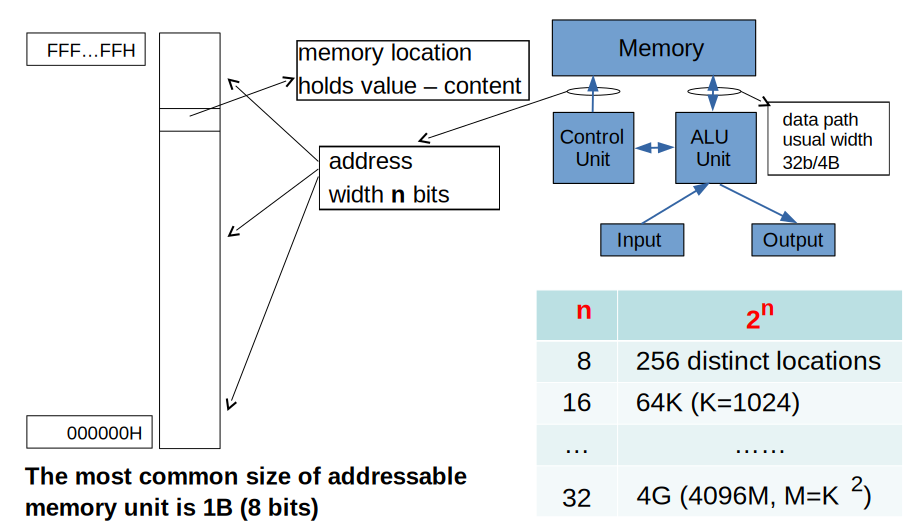
\includegraphics[width=.95\linewidth]{addr-space-en.pdf}

\end{frame}

\begin{frame}[shrink=2]
\frametitle{What is the Memory -- Description}

Memory:
\begin{itemize}
\item it is array of addressable memory cells
\begin{itemize}
\item all cells (elements) have the same size -- 8-bits (byte) is usual or multiple by two power
\end{itemize}
\item physical address space capacity is limited by number of bits forming address signal generated by CPU (ISA addressing modes) which are sent to address bus. For memory organize by bytes:
\begin{itemize}
\item 16-bit address allows to access cells in 64\,KiB of memory
\item 32-bit address allows to access  4\,GiB of memory capacity
\item 37-bit address (maximum for Intel Core  i9-13900K when mainboard support is as well) allows to address in 128\,GiB of capacity
\end{itemize}
\item Access types, rules:
\begin{itemize}
\item the internal memory of the computer allows access in random order (=~random access -- RAM)
\item some of external memory (for example magnetic tape used for backup -- cheaper than HDD and SSD) allows only sequential access, that is reading and writing of bytes in the fixed order
\item in HDD, SSD and Flash cases, only read or write by whole block is possible; for SSD/Flash is write possible on block basis and it is possible only once after much larger holding erase blocks is reset into initial consistent state.
\end{itemize}
\end{itemize}

\end{frame}

\begin{frame}
\frametitle{Semiconductor Memory -- Basic Terms}

\begin{description}
 \item[Address] input, it selects exactly one cell (entry) for next data read or write access (same as index for array in C language)
 \item[Value (data)] the corresponding cell data or signals to read or write them
 \item[control signals] set of signals choosing read or wrote operation, data validity, or used for redundancy which allows even bit-flip corrections
\end{description}

Main semiconductor memory parameters:

\begin{description}
  \item[Access time] (latency) the time interval from the request to data access to their availability to the requester
  \item[Read/write cycle time] access time (with precharge for DRAM) + refresh after destructive read + required idle time to next access
  \item[Throughput/bandwidth] main performance indicator. Rate of transferred data units per time.
  \item parameters can appear in the datasheet as maximal, average and minimal required
\end{description}

\end{frame}

\section{Semiconductor Memories -- HW Realization}

\begin{frame}
\frametitle{Memory Types and Required Maintenance}

Division of memories according to write operation mehanism:

\begin{itemize}
\item \textbf{ROM} (Read-Only Memory) memories that can only be read from (content defined ta production), include EEPROM (Electrically Erasable Programmable Read-Only Memory) requiring high voltage for erase and then allow write new data, write is not normal operation.
\item \textbf{RAM} (Random Access Memory) also RWM (Read-Write Memory) classic memories designed for reading and writing any cell in any order -- Random Access.
\end{itemize}

Division according data preservation when power is turned off and on:
\begin{itemize}
\item \textbf{Permanent} (Non-volatile) memory does not need power to keep information - e.g. Flash, EEPROM, EPROM, ROM, ferromagnetic memories, HDD, SSD, 3D-X Point -- Intel Optane Memory
\item \textbf{Volatile} (Volatile) for example DDR memory SDRAM, SRAM, cache in classical computer, continuous power (and data refresh for DRAM) is needed to maintain information.
\end{itemize}

\end{frame}

\begin{frame}
\frametitle{Memory Realization by Electrical Circuit}

According to the realization, we divide RAM (RWM) into:
\bigskip

\begin{tabular}{m{0.8cm}m{6cm}m{4cm}}
SRAM & Static RAM -- a physical quantity representing a value has a constant value over time. Typically two loop-connected inverters. Multiple components, more expensive, no periodic maintenance required, only needs power supply& 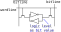
\includegraphics[width=3.8cm]{sram-en.pdf} \\
\phantom{x} & \\\
DRAM & Dynamic RAM -- a quantity (voltage) changes its value over time. Typically a capacitor that discharges spontaneously and therefore it is necessary to refresh the information at regular times. Only a capacitor and a transistor -- cheap, takes less space. & 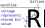
\includegraphics[width=3.2cm]{dram-en.pdf}\\\
\end{tabular}

Podle kontrukce dělíme paměti RAM (RWM) na:
\medskip

\begin{tabular}{m{0.8cm}m{6cm}m{4cm}}
SRAM & Statická RAM -- veličina reprezentující hodnotu má v čase konstatní hodnotu. Typicky dva do smyčky zapojené invertory. Více součástek dražší paměť, nemusí se obnovovat uložená informace, potřebuje pouze napájení & 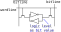
\includegraphics[width=3.8cm]{sram-en.pdf} \\
\phantom{x} & & \\
DRAM & Dynamická RAM -- veličina mění v čase svoji hodnotu. Typicky kondezátor, který se samovolně vybíjí a je proto nutné informaci obnovovat v pravidelných časech. Pouze kondenzátor a tranzistor -- levné, zabere méně prostoru. & 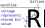
\includegraphics[width=3.2cm]{dram-en.pdf}\\
\end{tabular}

\end{frame}

\begin{frame}
\frametitle{Static Memory (SRAM) -- Cell Detail}

\hbox{
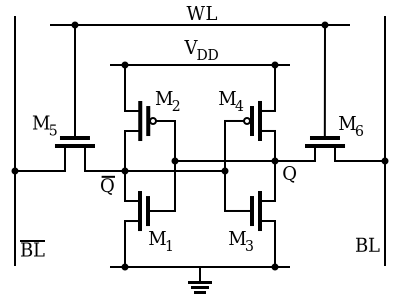
\includegraphics[width=0.4\linewidth]{sram-6t-cell.pdf}\hspace{0.1\linewidth}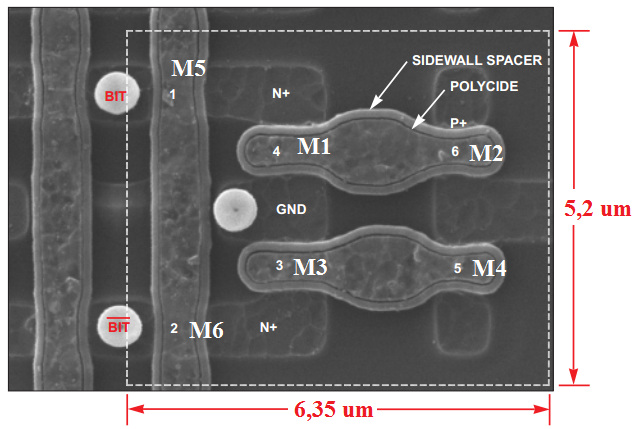
\includegraphics[width=0.4\linewidth]{fig/sram-cell.jpg}
}

\begin{itemize}
\item Fully static circuit (positive feedback)
\item Requires power supply (volatile memory) to maintain information
\item Disadvantage, needs 6 transistors, large area
\item Reading, after selecting a word (world line -- WL) the data is transferred to the respective non-powered conductor (bit line -- BL)
\item Writing -- connecting bit line and it inverted signal to log. 1 and log. 0 or vice versa will force the state with a greater current than on the inverter outputs in internal positive loop
\end{itemize}

\end{frame}

\begin{frame}
\frametitle{Dynamic memory (DRAM) -- Cell Detail}

\hbox{
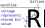
\includegraphics[width=0.4\linewidth]{dram-en.pdf}\hspace{0.1\linewidth}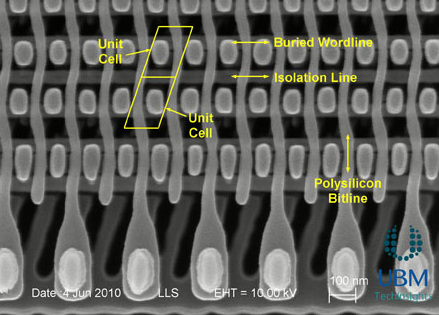
\includegraphics[width=0.4\linewidth]{fig/dram-cell.jpg}
}

\begin{itemize}
\item nMOS transistor represents a switch that connects (or not) the capacitor to the "bitline" conductor. The connection is controlled by the "wordline" conductor.
\item The reading process discharges the capacitor. Therefore, it must be restored afterwards.
\item Refreshing of memories (refresh) – the charge is spontaneously lost from the capacitor. Necessary working phase of dynamic memory. Negatively affects (prolongs) the average access time.
\end{itemize}

\end{frame}

\begin{frame}
\frametitle{Memory Array Organization -- the Principle}

\centering

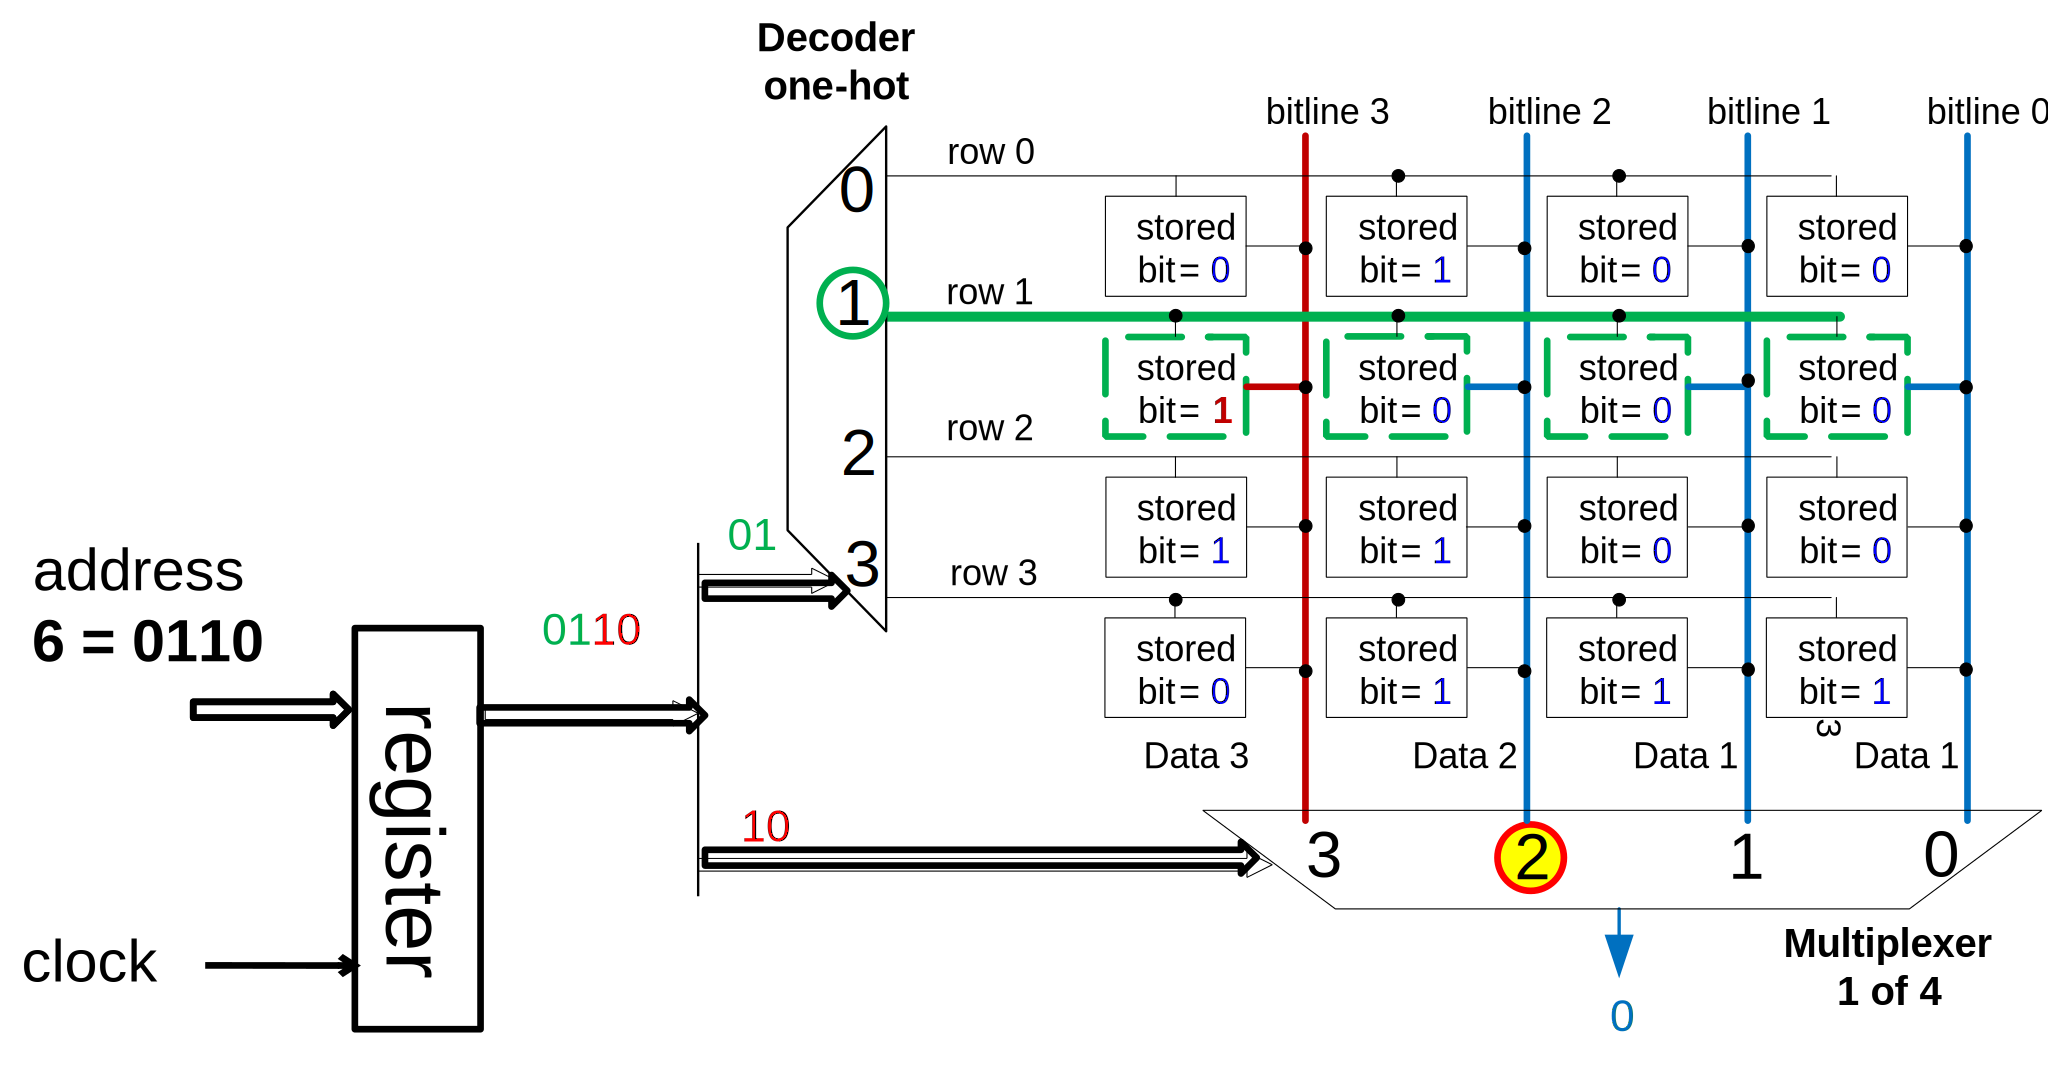
\includegraphics[width=1.0\linewidth]{ram-matrix.pdf}

\end{frame}

\begin{frame}
\frametitle{SDRAM Packaged as Dual In-Line Memory Module}

\centering

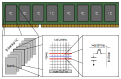
\includegraphics[width=0.75\linewidth]{sdram-dimm.pdf}

Dual In-Line Memory Module (DIMM), 64-bit data path, Synchronous Dynamic Random Access Memory (SDRAM), operation and signals synchronized (S in abbreviation) by clock

\end{frame}

\begin{frame}
\frametitle{}

{
\centering

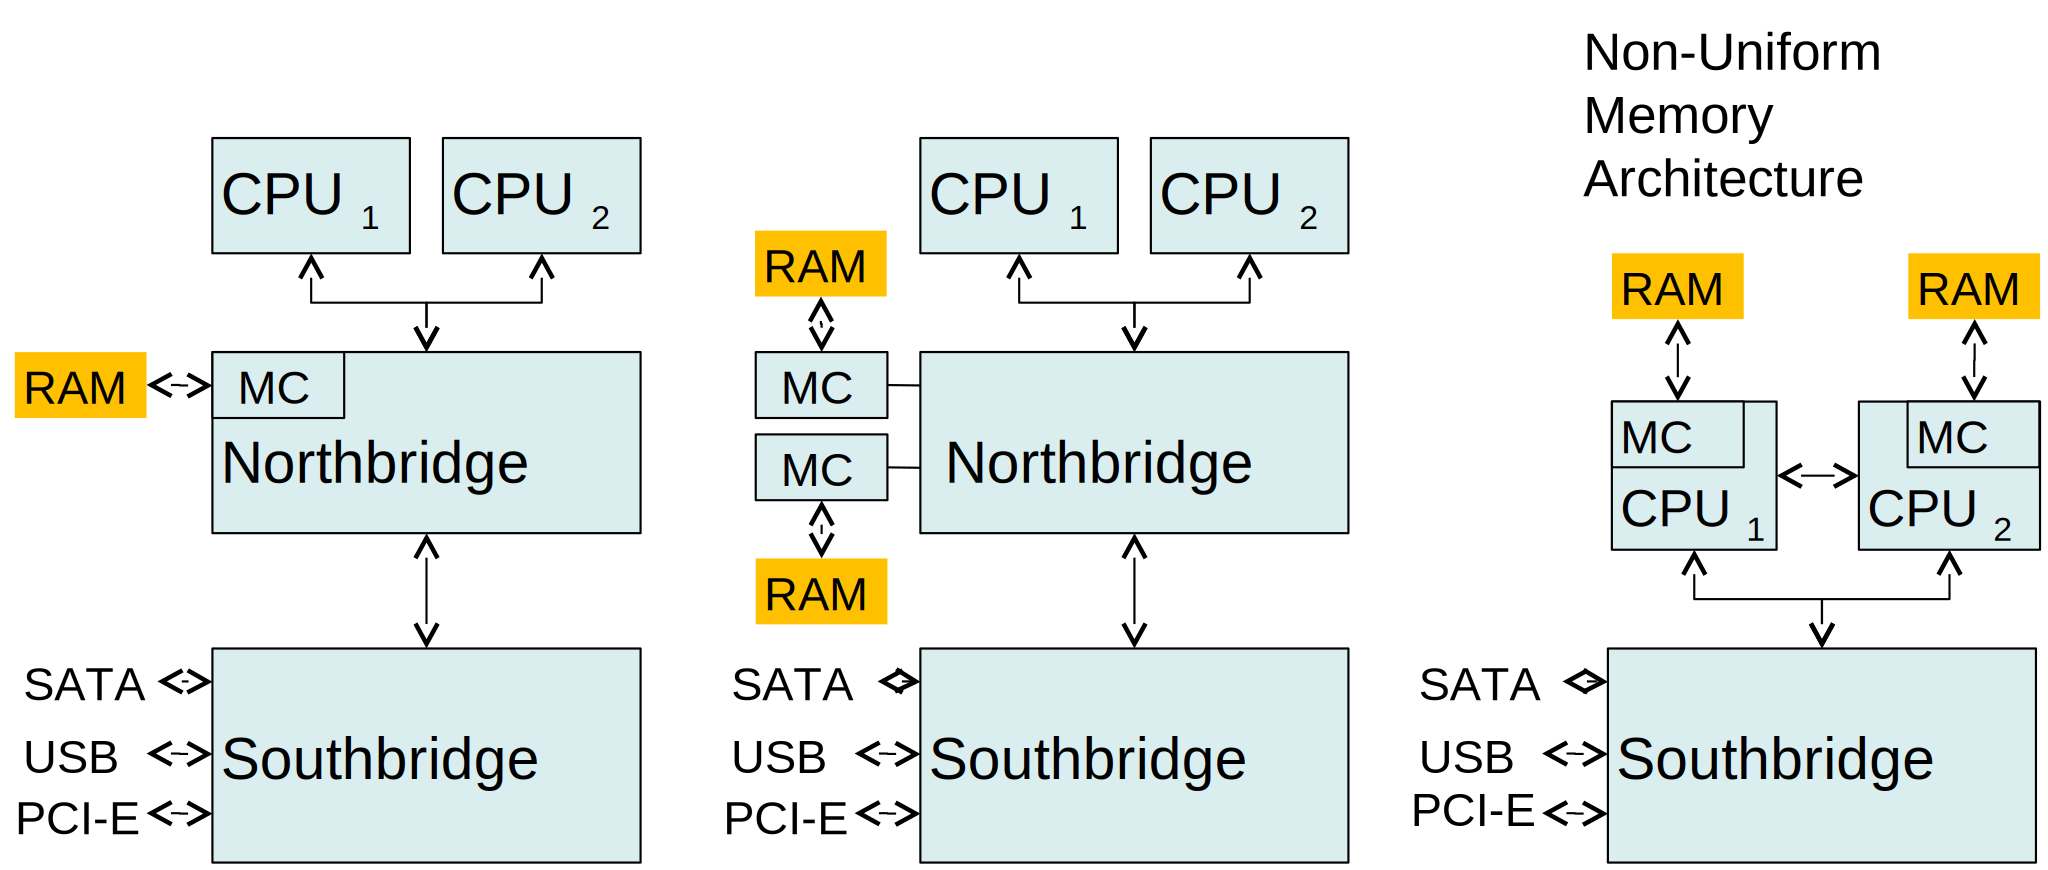
\includegraphics[width=0.85\linewidth]{pc-memory-to-numa.pdf}

}

\vskip 2mm

MC - Memory controller -- provides read and write control to SDRAM. It also controls refresh of information of each memory cell once every 64 ms typically (iterates over whole memory row by row and cells in each row are refreshed simultaneously).
\end{frame}


\begin{frame}
\frametitle{Most Frequently Used Dynamic Memory Types}

\begin{itemize}
\item \textbf{SDRAM} -- clock frequency up to 100 MHz, 2.5V, synchronous data transfer on the clock edge
\item \textbf{DDR SDRAM} -- data transfer on both clock signal edges, 2.5V, I/O clocks up to 100-200 MHz, 0.2-0.4 GT/s (billions of transmissions per skund)
\item \textbf{DDR2 SDRAM} -- lower power consumption, 1.8V, frequency up to 400 MHz, 0.8 GT/s
\item \textbf{DDR3 SDRAM} -- even lower power consumption at 1.5V, frequency up to 800 MHz, 1.6 GT/s
\item \textbf{DDR4 SDRAM} -- 1.05 -- 1.2V, I/O bus clock 1.2 GHz, 2.4 GT/s
\item \textbf{DDR5 SDRAM} -- 1.1V, up to 6.4 GT/s
\end{itemize}

All of these types are predominantly optimized for throughput, not random access, latency 20 to 35 ns.

\end{frame}


\begin{frame}
\frametitle{Memory and CPU Speed Evolution in History}

\centering

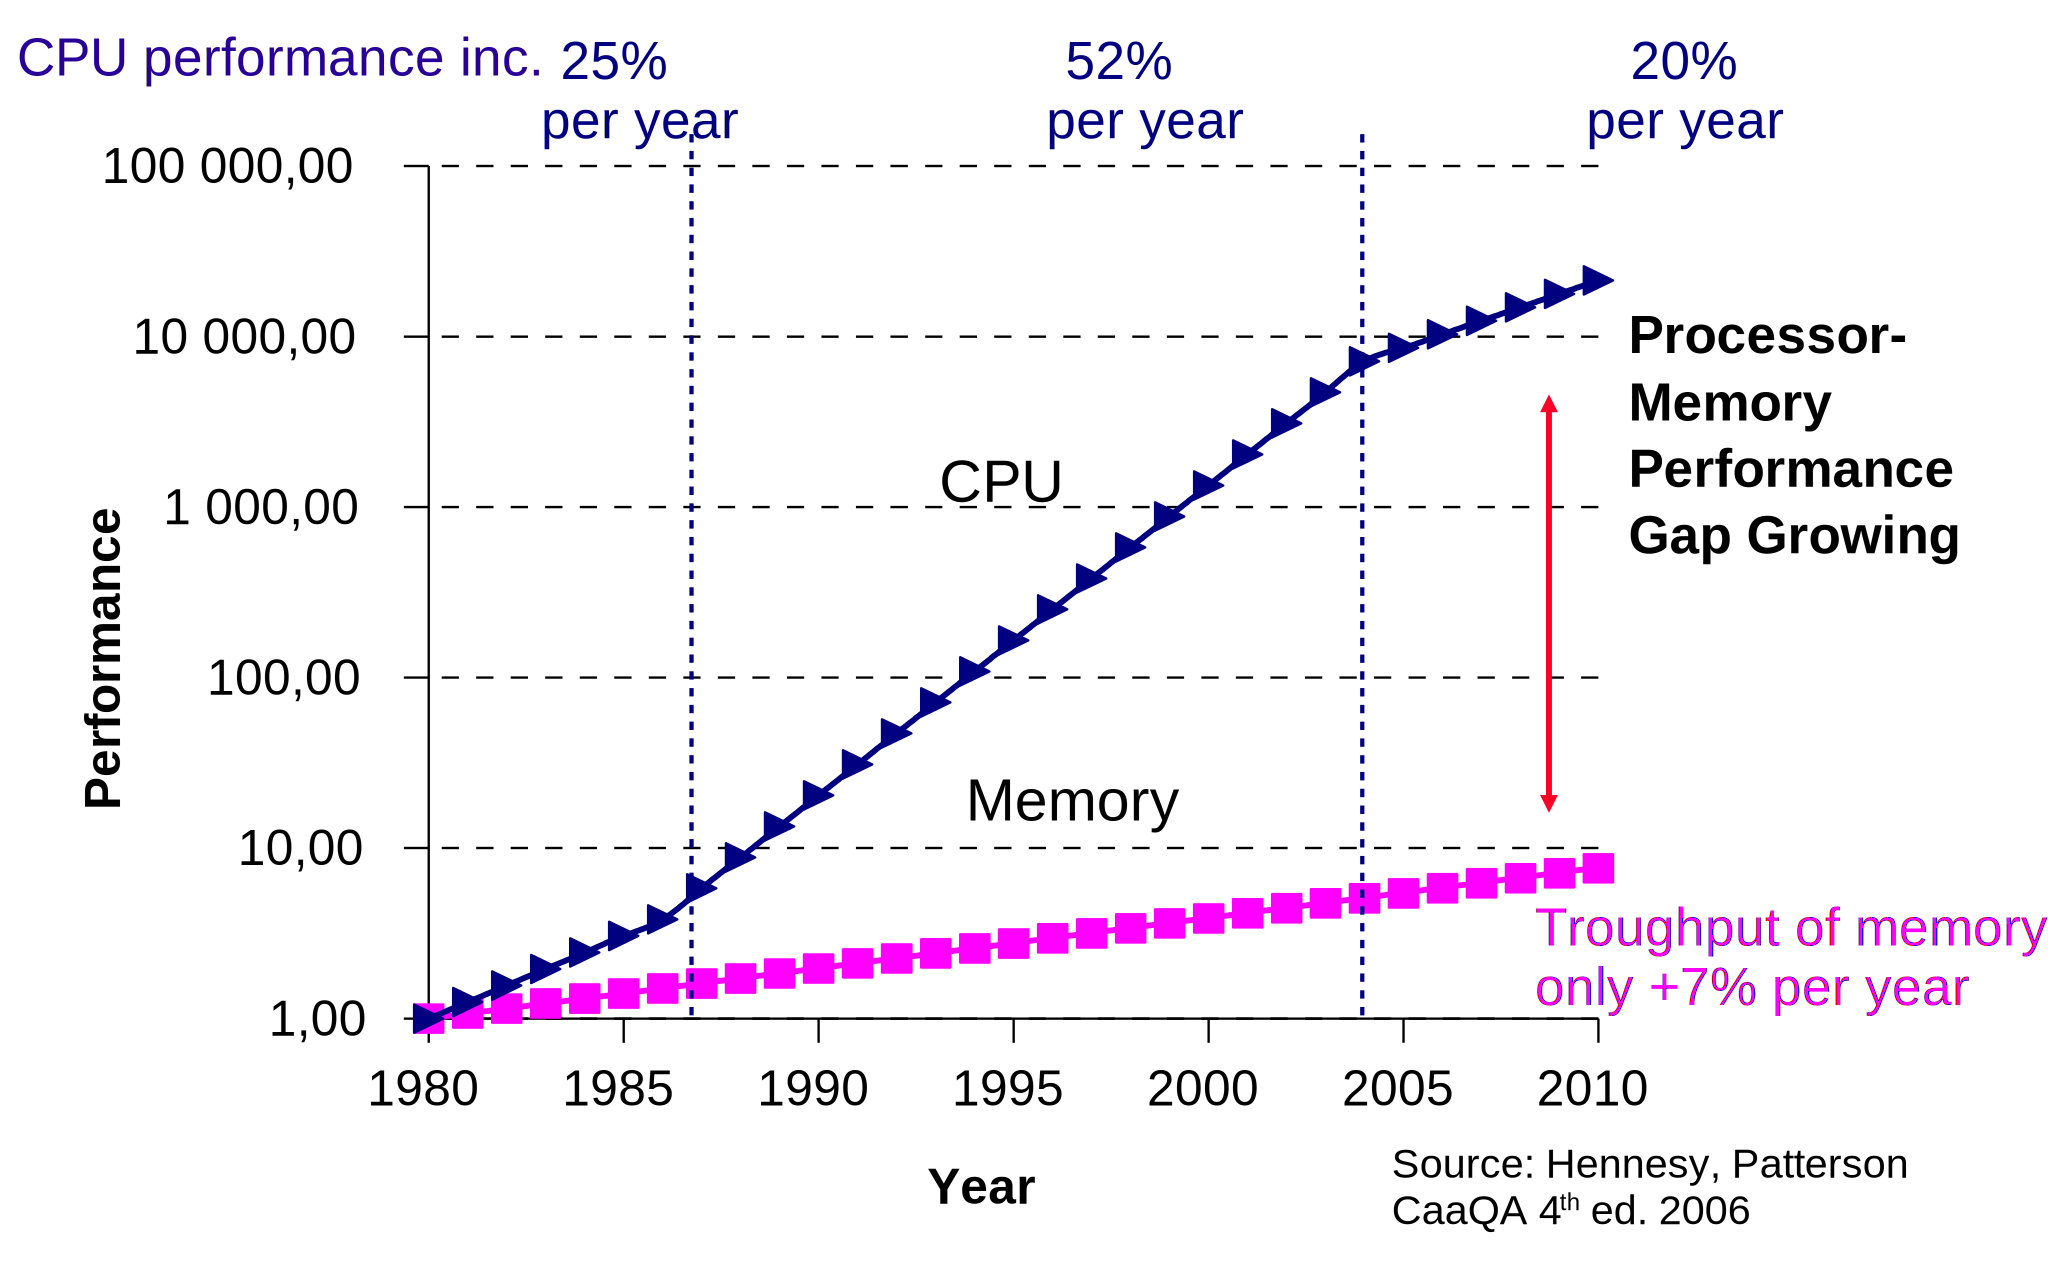
\includegraphics[width=1.0\linewidth]{memory-gap-en.pdf}

\end{frame}

\section{Cache Memory to Speed Up Data Access}

\begin{frame}
\frametitle{Memory Hierarchy from CPU Registers to SSD}

{
\centering

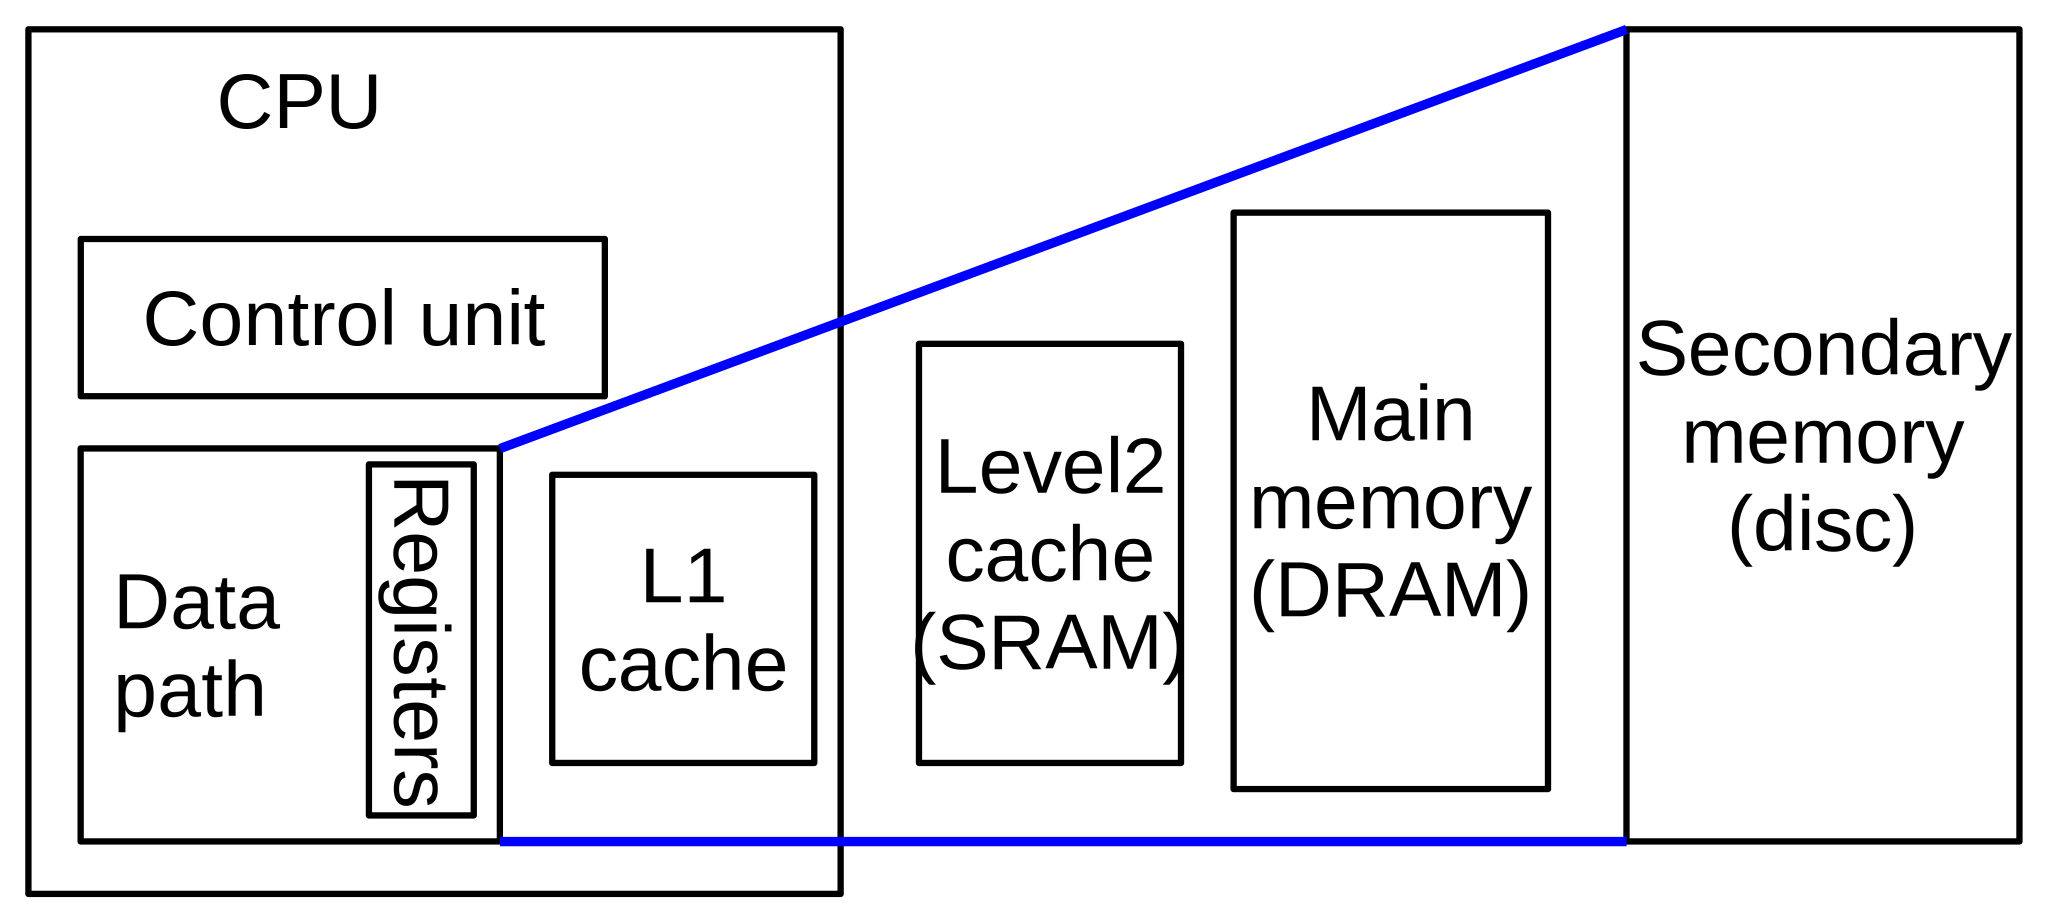
\includegraphics[width=0.65\linewidth]{mem-reg-to-disc.pdf}

}
\vskip 2mm

\begin{tabular}{l|llll}
Type     & L1 SRAM   & Sync SRAM &  DDR3      & HDD \\
Velikost & 32kB      & 1 MB      &  16 GB     & 3TB \\
Cena     & 10 kč/kB  & 300 kč/MB &  123 kč/Gb & 1 kč/GB \\
Rychlost & 0.2...2ns & 0.5...8 ns/word & 15 GB/sec & 100 MB/sec \\
\end{tabular}

\vskip 2mm

Some data may exist in multiple copies (levels, SMPs).
Modifying data requires mechanisms to maintain the coherence (mostly by HW) of words and consistency of data structures (programmer care required).

\end{frame}

\begin{frame}
\frametitle{Memory Hierarchy -- Fundamental Principles}

\begin{itemize}
\item Programs/processes access only a small portion of their address space at a time
\item \textbf{Temporal locality}
\begin{itemize}
\item Items accessed recently will be needed again soon
\item Example: program loop, function local and induction variables
\end{itemize}
\item \textbf{Spatial locality}
\begin{itemize}
\item Items near those accessed recently are likely to be accessed soon
\item Example: sequence code access (program memory), data arrays sequential access (data memory).
\end{itemize}
\end{itemize}
The principle considered on all levels, in algorithms (local variables), compilers (move to registers), between memory levels (automatically), operating system (move pages between disk and main memory) or again programmatically, reading and writing to files or caching web pages.

\end{frame}


\begin{frame}
\frametitle{Memory Hierarchy Introduced Based on Locality}

\begin{itemize}
\item The solution to resolve capacity and speed requirements is to build address space (data storage in general) as hierarchy of different technologies.
\item Store input/output data, program code and its runtime data on large and cheaper secondary storage (hard disk)
\item Copy recently accessed (and nearby) items from disk to smaller DRAM based main memory (usually under operating system control)
\item Copy more recently accessed (and nearby) items from DRAM to smaller SRAM memory (cache) attached to CPU (hidden memory, transactions under HW control), optionally, tightly coupled memory under program's control
\item Move currently processed variables to CPU registers (under machine program/compiler control) 
\end{itemize}

\end{frame}


\begin{frame}
\frametitle{Cache Memory to Overcome CPU Speed Growth Gap}

\begin{itemize}
\item component that (transparently) stores data so that future requests for that data can be served faster
\item transparent cache – hidden memory
\item the purpose of hidden memory is to speed up access to frequently used data on "slow" media by copying it to fast media.
\item it mostly works automatically and adapts to the current needs of the program.
\item however, it is necessary to know about its existence and often needs servicing at the level of the operating system and, in some cases, even programs.
\item if you choose data structures, access paterns and algorithms unwisely, its effect is lost.
\end{itemize}

\end{frame}

\begin{frame}[shrink=1]
\frametitle{Cache Memory -- Terms Definition}

\begin{itemize}
\item \textbf{Cache hit} naming the situation when the data for requested address is found in the cache.
\item \textbf{Cache miss}, opposite, \textbf{search failure}, the data is not yet in the cache.
\item \textbf{Cache line} (line) or \textbf{Cache block} – the basic copieable unit between hierarchical levels.
\item In practice, the size of the \textbf{Cache} line varies from 8B to 1KB, typically 64B.
\item \textbf{Hit rate} -- the number of memory accesses served by a given cache level divided by all accesses
\item \textbf{Miss rate} -- the ratio of accesses to be served from slower memory = 1 - Hit rate
\item \textbf{Average Memory Access Time} (AMAT) $$AMAT = Hit Time + Miss Rate \times Miss Penalty$$
\item AMAT for multi-level cache can be calculated by recursively applying the aforementioned relationship
\end{itemize}

\end{frame}

\begin{frame}[shrink=1]
\frametitle{Cache Memory -- Implementation}
{
\centering

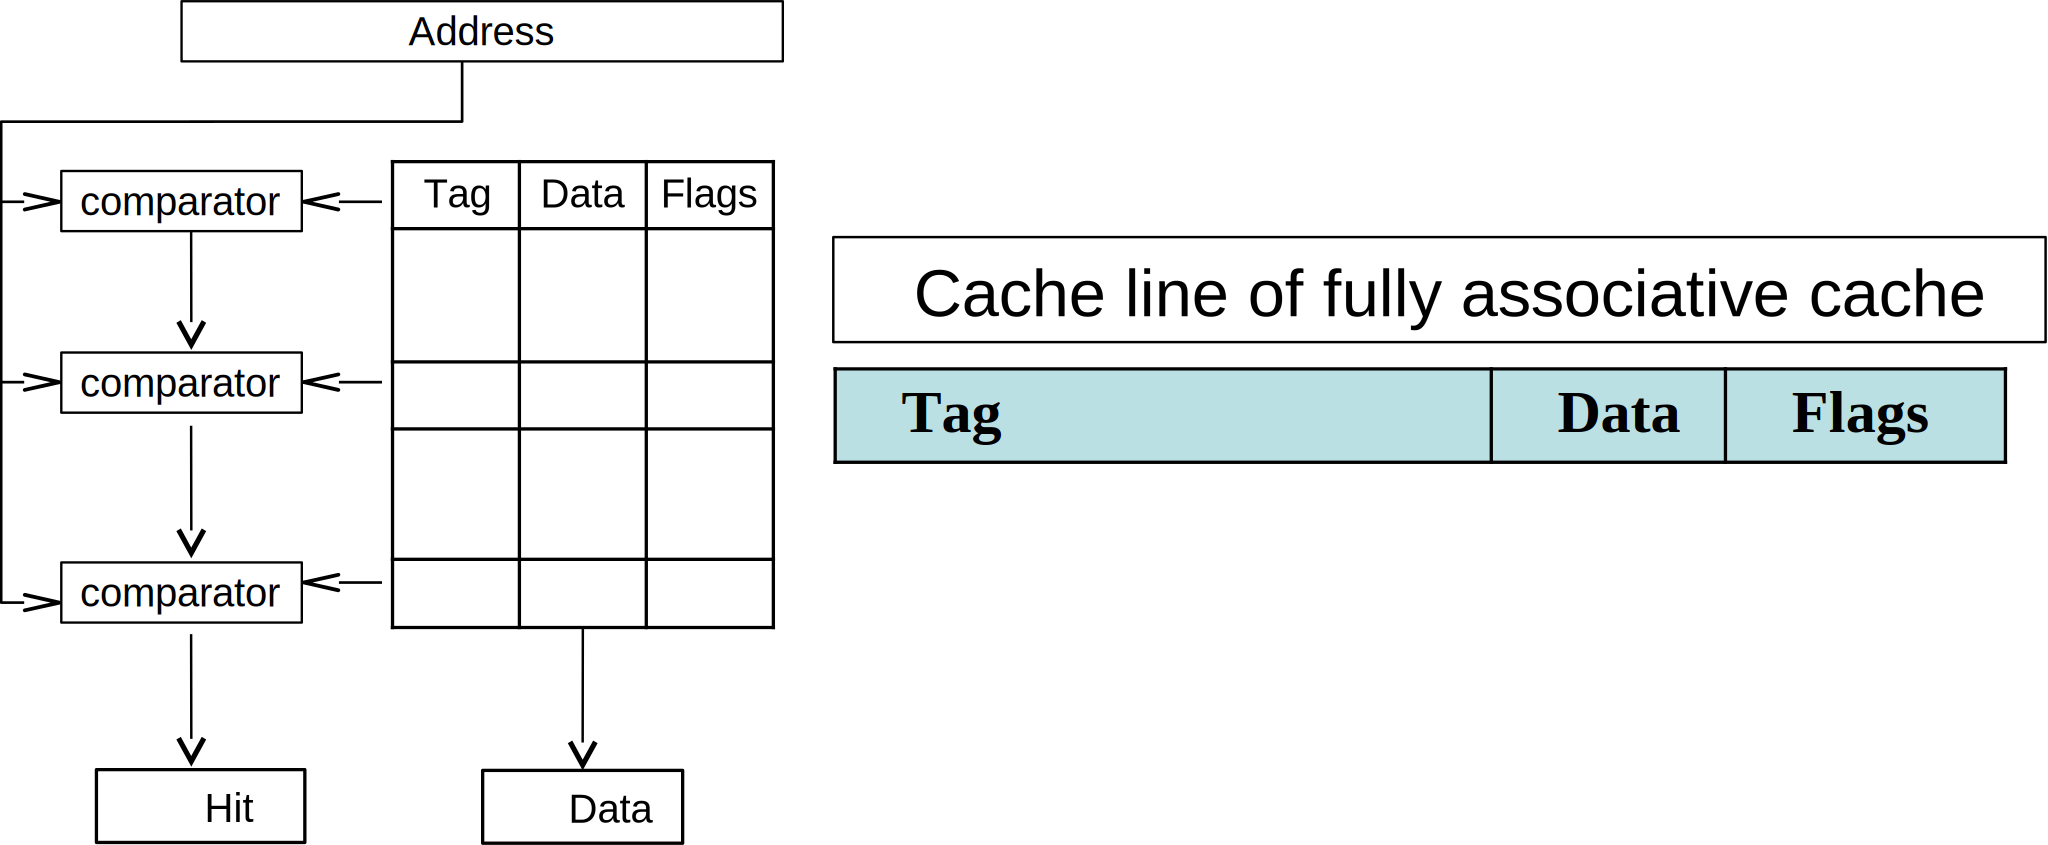
\includegraphics[width=0.75\linewidth]{cache-principle.pdf}

}
\vskip 2mm

\begin{itemize}
\item \textbf{Tag} is the index of the corresponding block in the operating memory (basically, it is the value of the pointer/address divided by the length of the block or cache way -- see later).
\item \textbf{Data} is an array containing actual values at the corresponding address(s).
\item \textbf{Validity bit} – indicates whether the contents of the \textbf{Data} field are even valid.
\item \textbf{Dirty bit} –  indicates that there is a different value in the cache than in the main memory.
\item more additional bits (metadata) attached to memory content can be required for SMP and maintenance
\end{itemize}

\end{frame}


\begin{frame}
\frametitle{Processing of Cache Miss Situation}

\begin{itemize}
\item Data must be loaded from main memory, but usually all cache entries are already filled with data retained from a previous run of the program.
\item One of the blocks that can be used to store data from the given address needs to be released.
\item Deciding an block to discard is very important, if the one that will be needed again is selected, performance will decrease.
\item \textbf{Cache replacement policy} -- rules for selecting an item to discard
\begin{itemize}
\item \textbf{Random} -- the selected block is at random position in the cache
\item \textbf{LRU} (Least Recently Used) -- the selected block is the longest unused one, additional information must be added to the cache circuits to each block group to track the order of recent hits for each item.
\item \textbf{LFU} (Least Frequently Used) -- tracks how often/how many times the blocks are accessed, requires adding forgetting.
\item \textbf{ARC} (Adaptive Replacement Cache) - combination of LRU and LFU
\end{itemize}
\end{itemize}

\end{frame}


\begin{frame}
\frametitle{Processor Writes to Cached Main Memory}

\begin{itemize}
\item Cache is on the way that may contain the block being written to.
\item At least from the point of view of the given processor, it is necessary to ensure the data coherence for the given processor (often for multiple processors -- threads) for accessing each individual address even if there are multiple access paths
\item \textbf{Write through} cache -- if the data is already in the cache, it is modified, in the variant with automatic allocation, block is loaded and then modified even if there is a miss. The data is sent to the main memory at the same time, either directly or via write buffer
\item \textbf{Write back} -- the data is written to the appropriate cache block, if it is not in the cache, the block is loaded first. The block is marked by \textbf{Dirty bit}. Writing to the next level is activated only if the cache entry needs to be released for replacement of other data or when sychronization by is requested by the processor, system (cache flush) is required.
\end{itemize}

\end{frame}

\begin{frame}
\frametitle{Basic Cache Organization Configurations}

We consider a cache of 8 blocks and situation where main memory block at address/block\_size equal to 12 is acessed. Which cache block(s) can be used for this situation

\bigskip

\begin{tabular}{p{0.29\linewidth}p{0.29\linewidth}p{0.29\linewidth}}
\textbf{Fully Associative} & \textbf{Direct Mapped} & \textbf{2-Way Associative} \\
Address 12 can be placed arbitrarily &
Address 12 can be placed only in block 4 (12 mod 8) &
Address 12 can be placed in set 0 (12 mod 4) \\
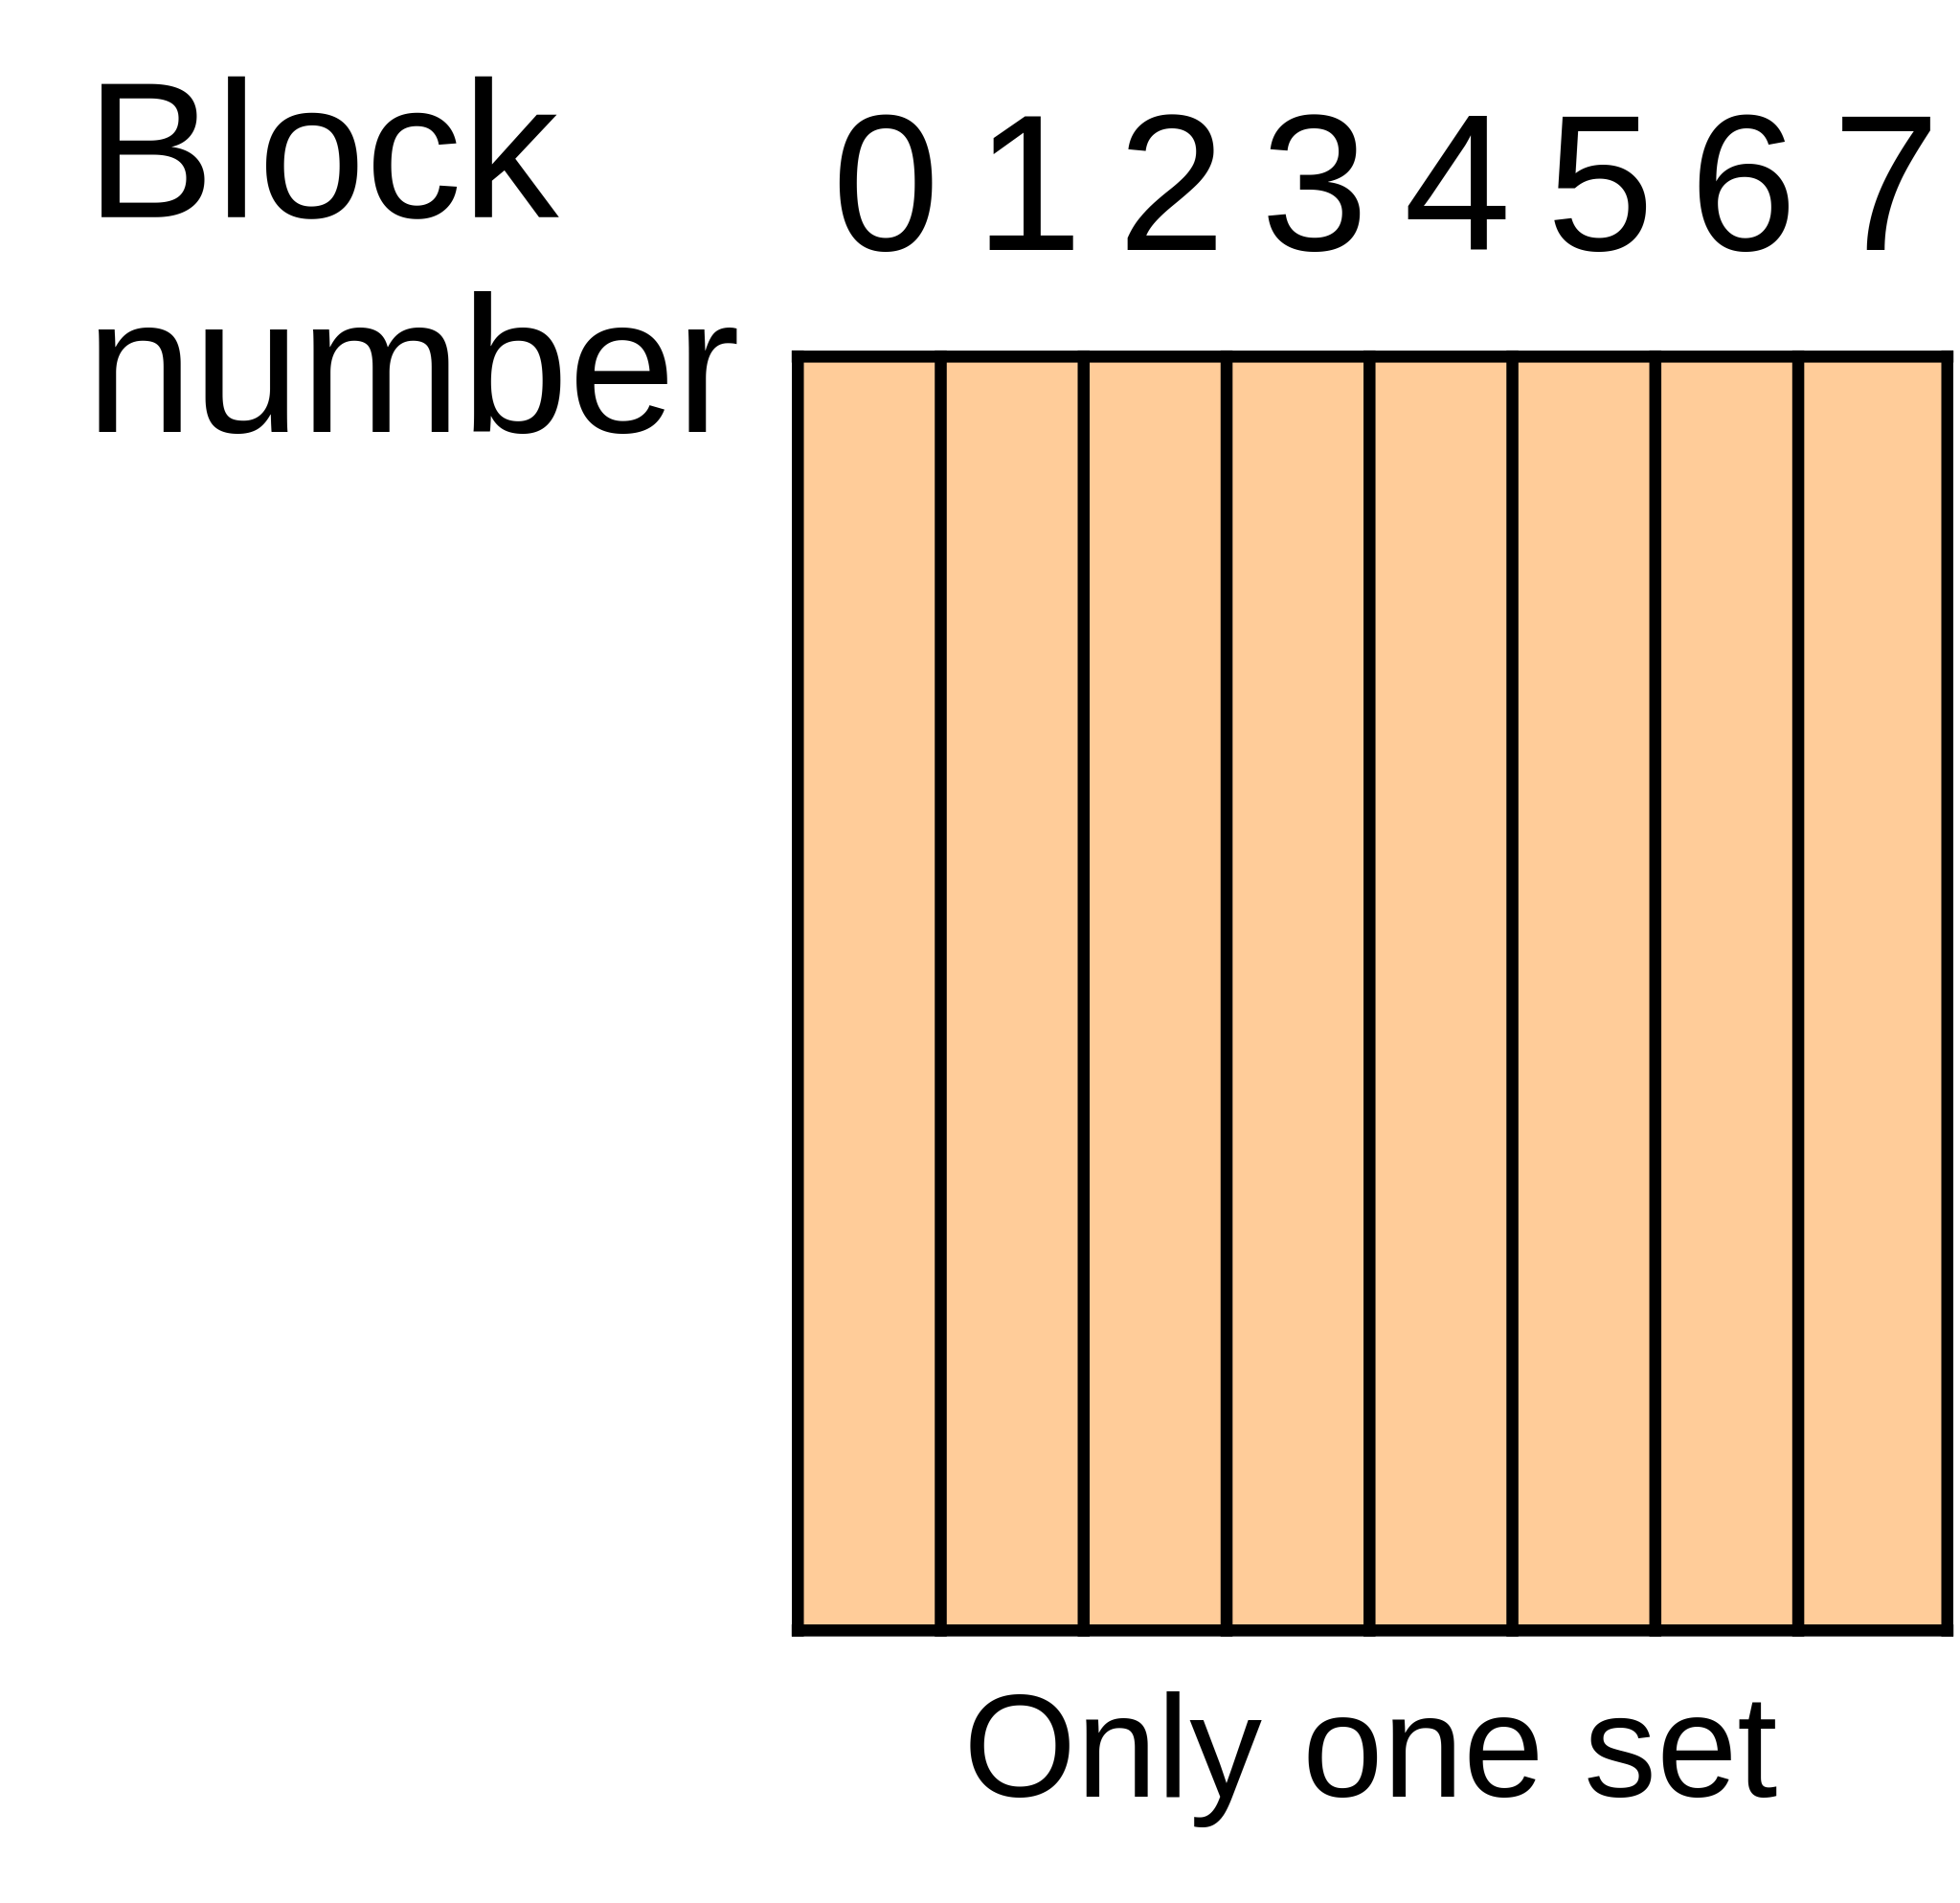
\includegraphics[width=3cm]{cache-schema-fully.pdf} &
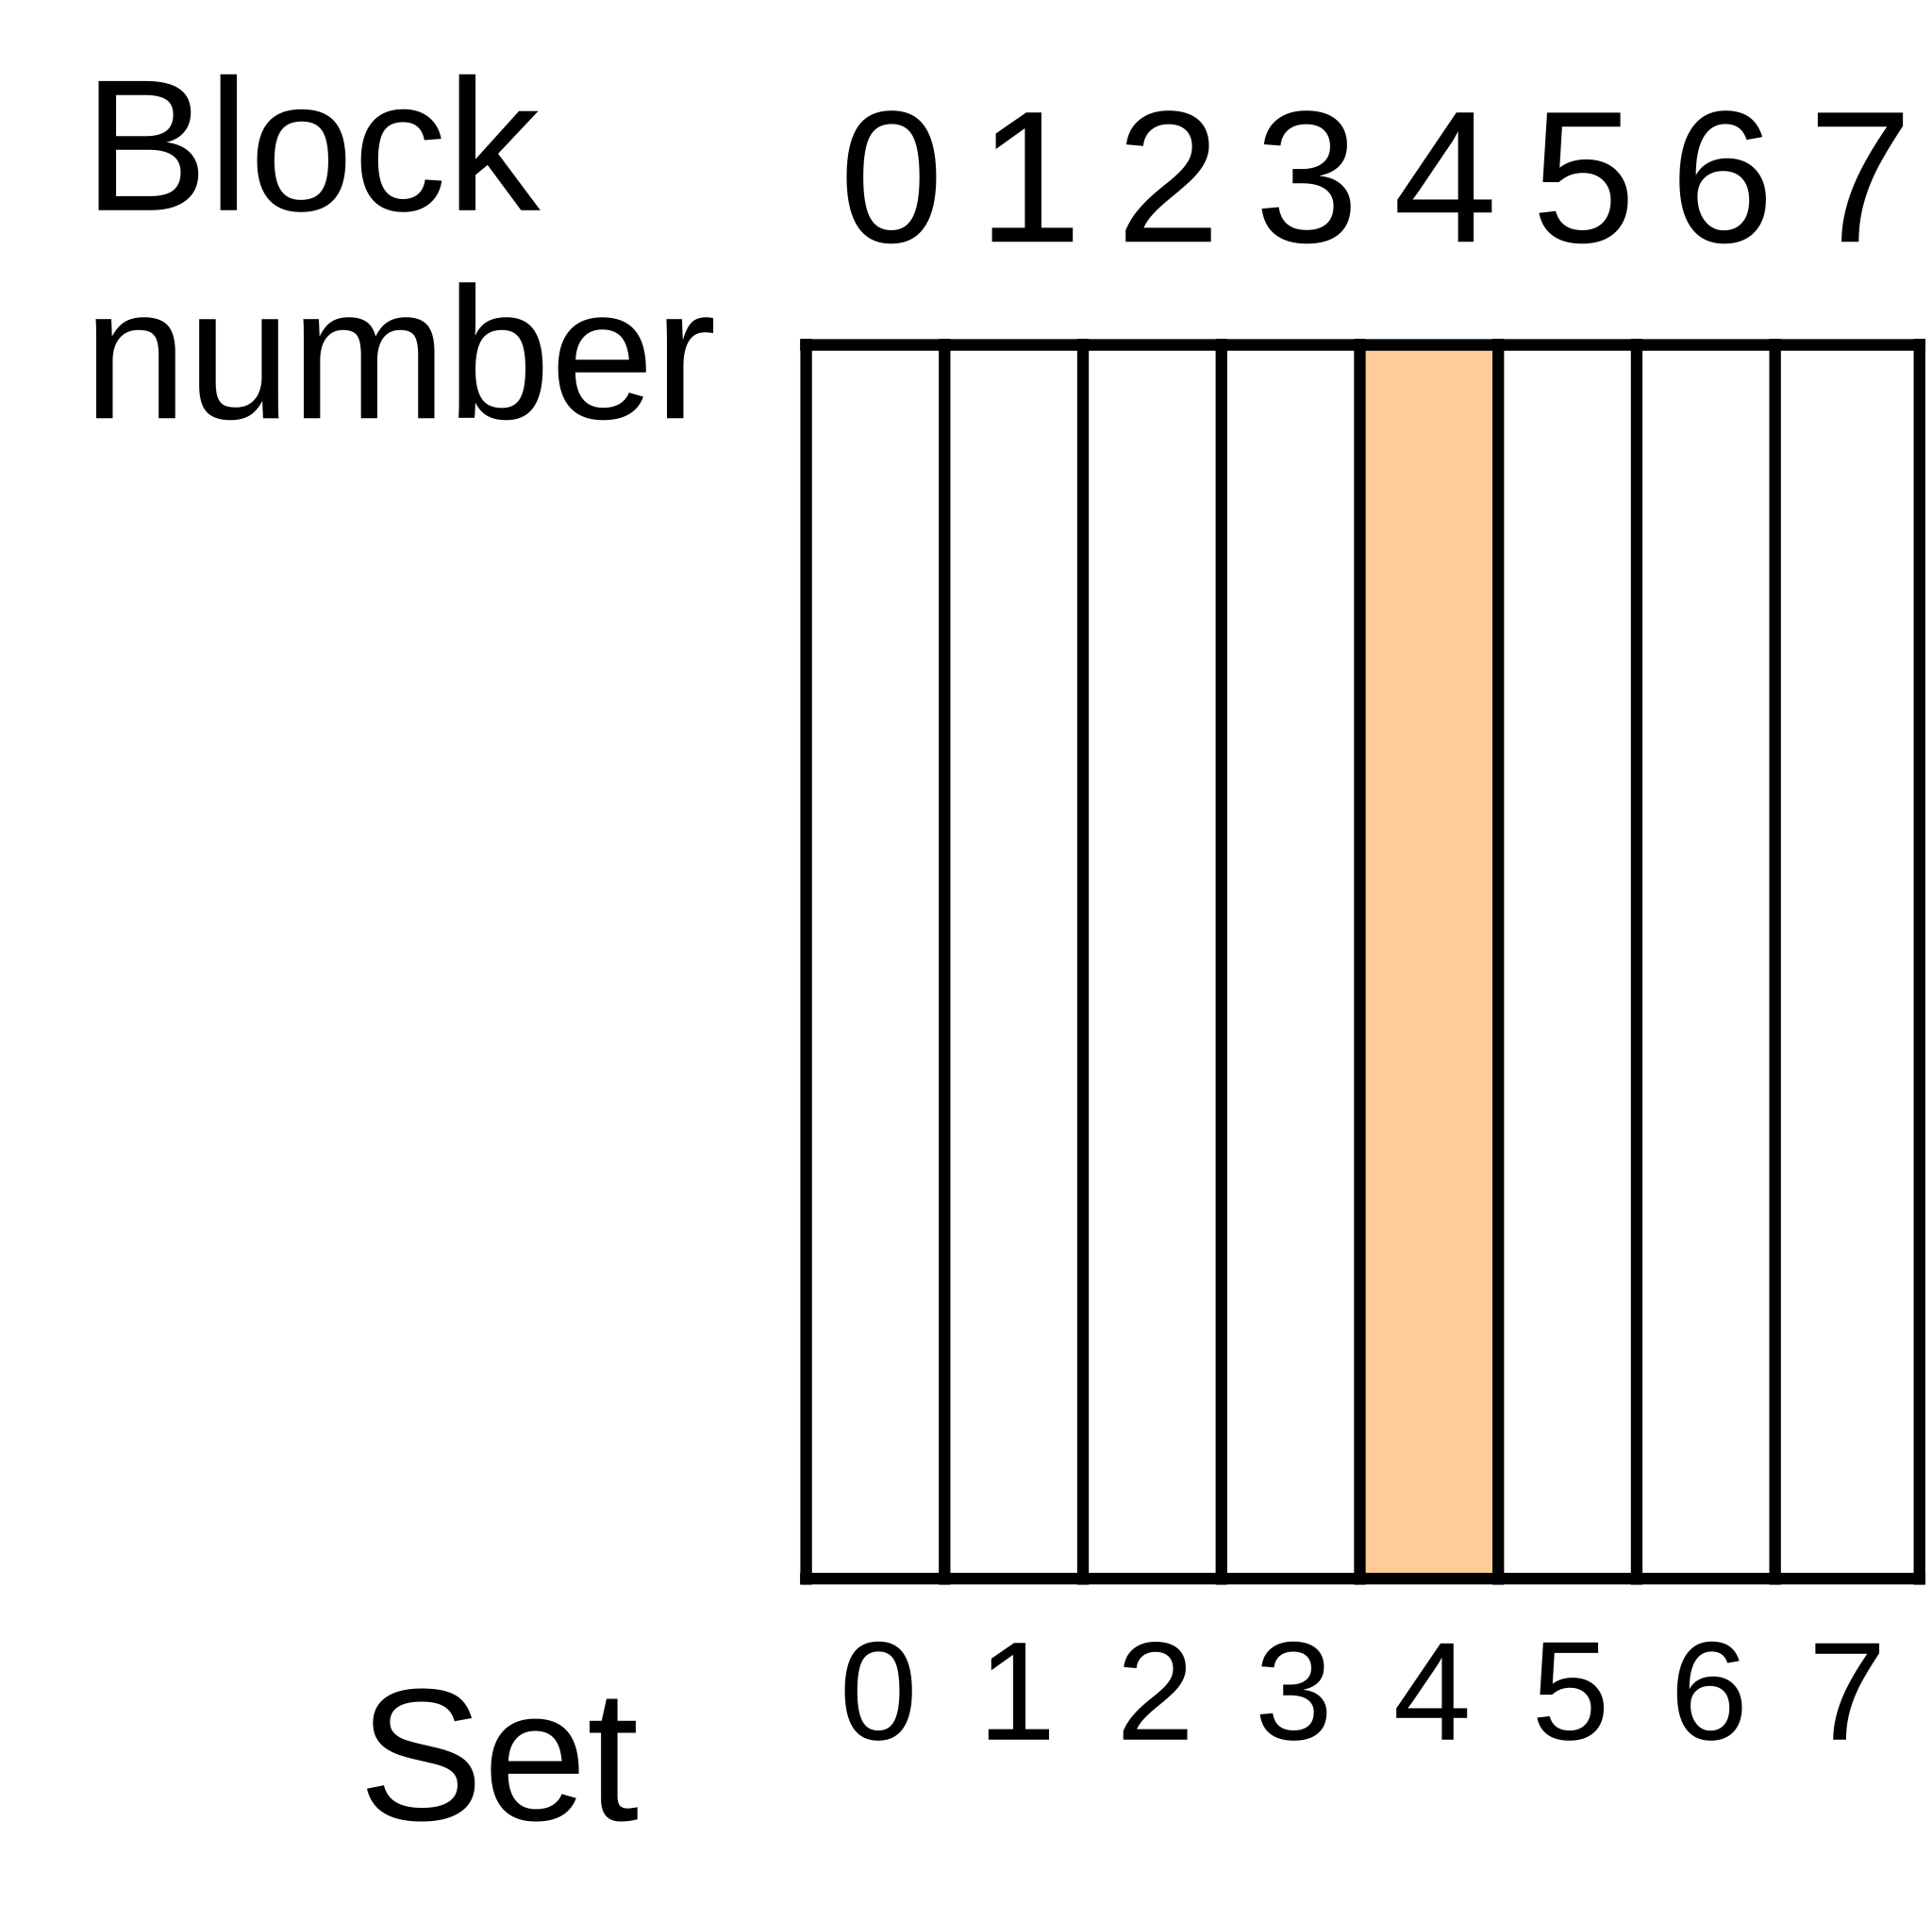
\includegraphics[width=3cm]{cache-schema-direct.pdf} &
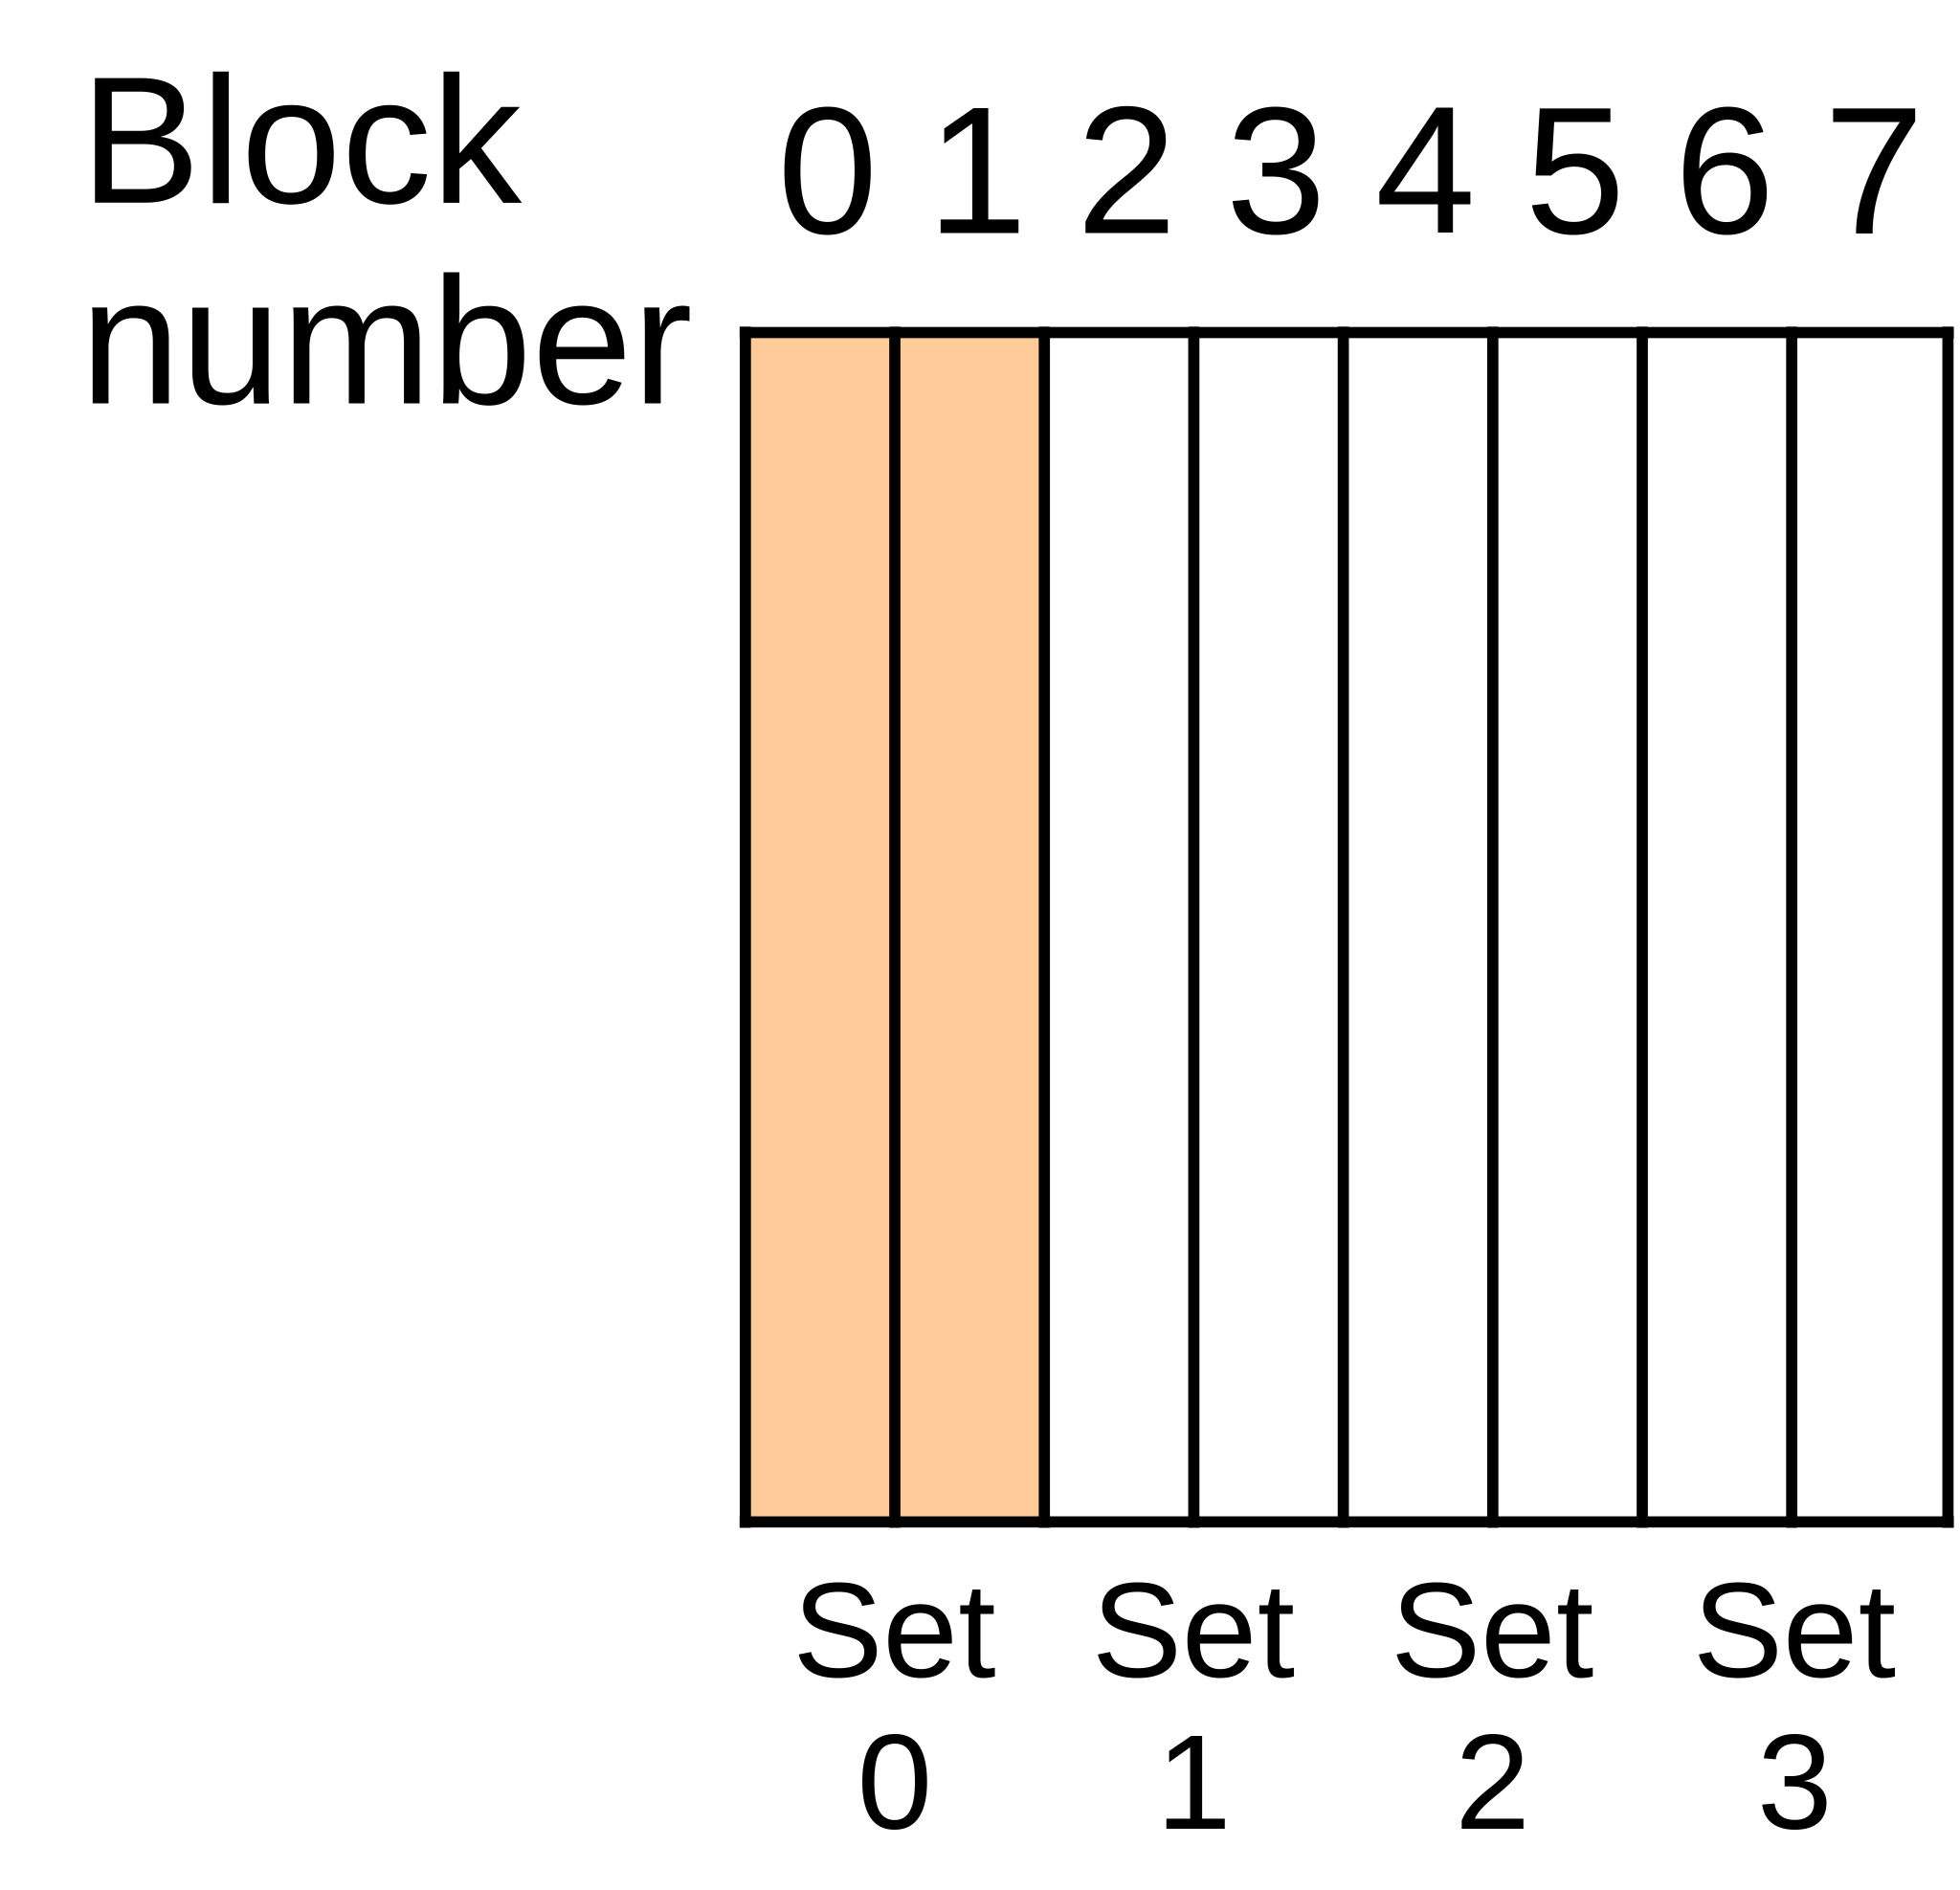
\includegraphics[width=3cm]{cache-schema-2way.pdf} \\
\end{tabular}

\end{frame}

\begin{frame}
\frametitle{Direct Mapped Cache Memory -- Mapping of Addresses}

{
\centering

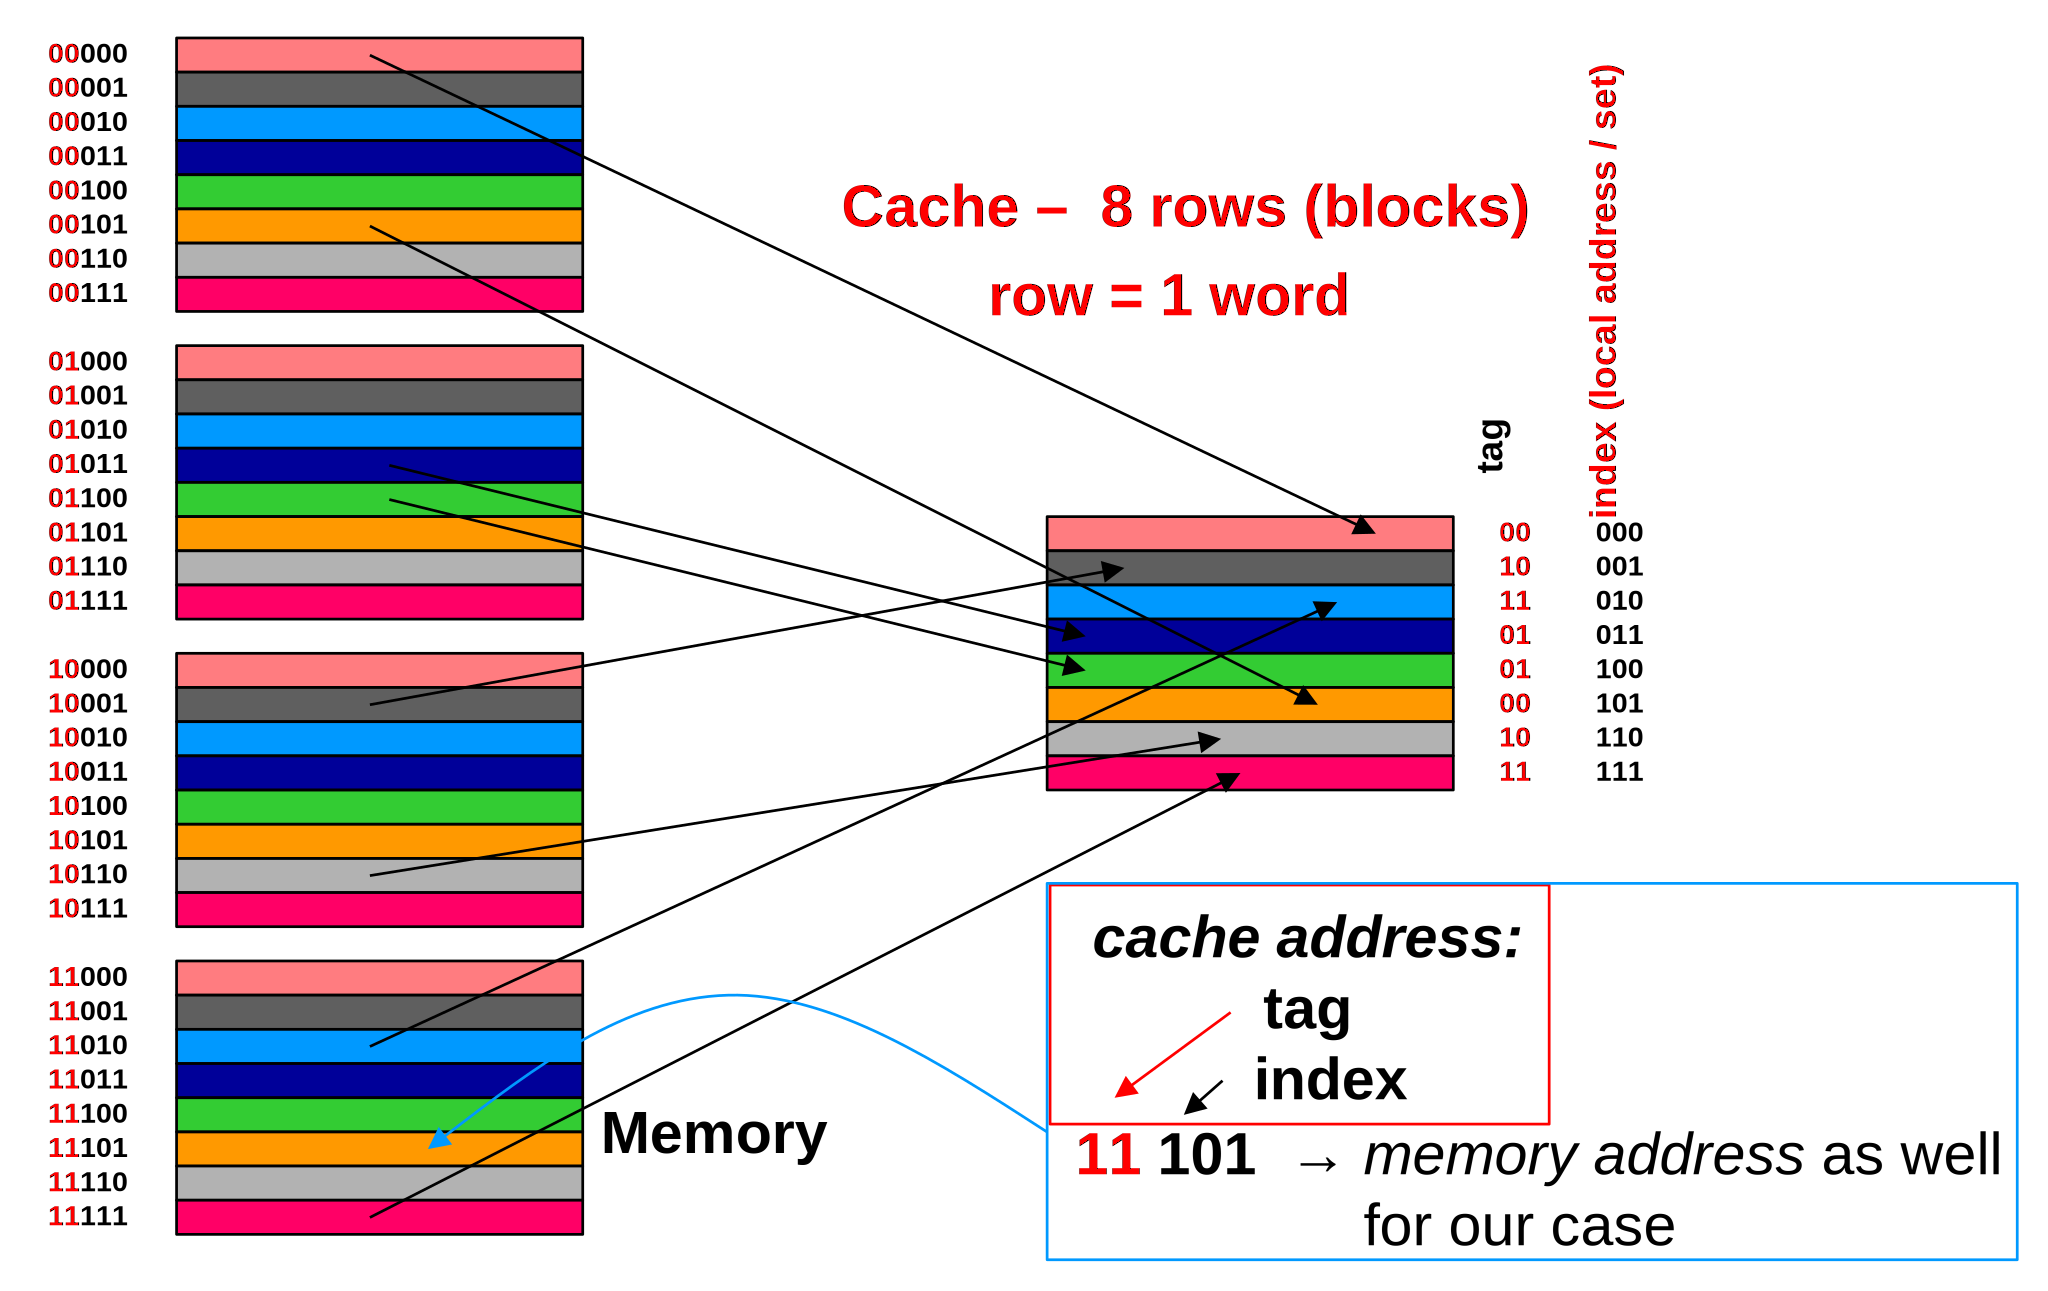
\includegraphics[width=0.9\linewidth]{cache-direct-mapping-1byte.pdf}

}

\end{frame}

\begin{frame}
\frametitle{Direct Mapped Cache Memory for Block Equal to Word}

\begin{itemize}
\item \textbf{Capacity} -- C ... in figure 1024 bytes which is 256 words
\item \textbf{Number of sets} -- SN .. 256 sets (equal to $C/WS/BS$)
\item \textbf{Word size} – WS .. 4 bytes for considered example
\item \textbf{Block size} – BS .. 1 word (4 bytes) for shown example
\item \textbf{Number of blocks} -- BN .. number of blocks (256 there)
\item \textbf{Degree of associativity} -- N number of ways to which capacity or blocks are divided (1 there)
\end{itemize}

{
\centering

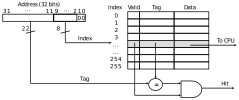
\includegraphics[width=0.70\linewidth]{cache-direct-simple.pdf}

}

C = 1024 bytes, SN = BN = 256, BS = 1, N = 1

\end{frame}


\begin{frame}
\frametitle{Direct Mapped Cache Memory for Larger Block Size}

BS = 4 (16 byte, word WS = 4 byts), number of sets SN = 4

set = (adresa div BS) mod SN

{
\centering

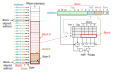
\includegraphics[width=0.75\linewidth]{cache-direct-ms.pdf}

}

{\tiny Source: Michal Štepanovský}
\end{frame}

\begin{frame}
\frametitle{General Cache Memory Organization with N Ways}

{
\centering

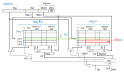
\includegraphics[width=0.95\linewidth]{cache-n-way-ms.pdf}

}

{\tiny Source: Michal Štepanovský}

\end{frame}

\begin{frame}
\frametitle{Demonstration: QtRvSim vect-inc, vect-add2, vect-add}

Start with direct mapped cache and \texttt{vect-inc}. If the block size is greater than one word and the vector size is greater than the capacity of one path, \texttt{vect-add2} will experience considerable performance degradation. After increasing the degree of associativity to two ways even while maintaining the overall capacity, aliasing does not occur anymore. However, after extending the algorithm to work with three vectors (\texttt{vect-add}), the cache trashing occur again for write-back or write- through and allocate setup. The worst situation will occur for the LRU policy. Increasing the degree to three, or rather to the more usual four, ways will again suppress the number of misses to one for each sequentially accessed block.

\begin{itemize}
\item \url{https://gitlab.fel.cvut.cz/b35apo/stud-support/-/tree/master/seminaries/qtrvsim/vect-inc}
\item \url{https://gitlab.fel.cvut.cz/b35apo/stud-support/-/tree/master/seminaries/qtrvsim/vect-add2}
\item \url{https://gitlab.fel.cvut.cz/b35apo/stud-support/-/tree/master/seminaries/qtrvsim/vect-add}
\end{itemize}

\end{frame}

\begin{frame}
\frametitle{Miss Rate and Cache Organization and Size Relations}

{
\centering

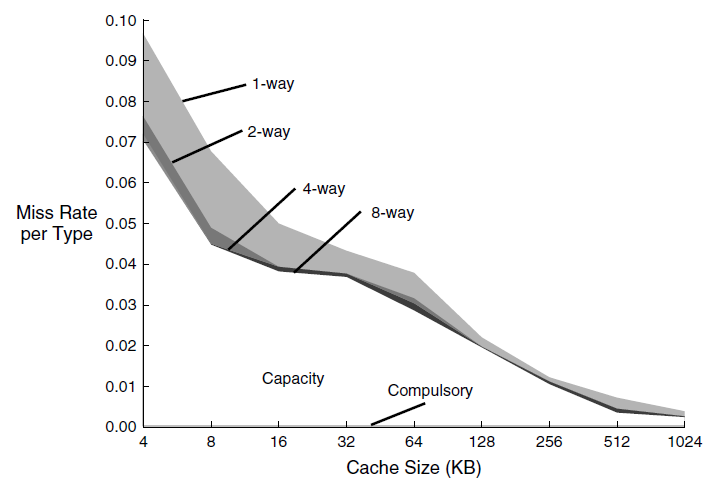
\includegraphics[width=0.65\linewidth]{cache-size-vs-ways.pdf}

}

\begin{itemize}
\item miss rate is not cache parameter/feature
\item miss rate is not parameter/feature of the program/algorithm
\end{itemize}

Miss rate depends on both the algorithms in the program and the cache parameters
and often the data being processed.
\end{frame}

\begin{frame}
\frametitle{Miss Rate Changes with Cache capacity and Block Size}

Miss rate versus block size and cache size on SPEC92 benchmark

\vskip 2mm

{
\centering

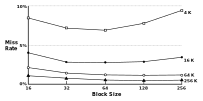
\includegraphics[width=0.72\linewidth]{cache-size-vs-block.pdf}

}

\vskip 2mm

{\tiny Source: Hennessy and Patterson: Computer Architecture: A Quantitative Approach 3rd ed., Morgan Kaufmann, 2003}

Increasing block size helps to load neighboring data, which would often subsequently be needed.
But if additional cached date are not needed, then the cache miss penalty increases and at the same time there are more collisions and cache capacity is wasted for unnecessary data.

\end{frame}


\begin{frame}
\frametitle{Miss Rate Changes with Cache capacity and Block Size}

\begin{enumerate}
\item Larger block size \\ Reduces compulsory misses; increases other misses, miss penalty
\item Larger cache size \\ Reduces capacity/conflict misses; increases hit time, power, cost
\item Greater associativity \\ Reduces conflict misses; increases hit time, power
\item Multiple cache levels \\ Reduces Miss Penalty, allows for optimizations at each level
\item Prioritize read misses over writes
\item Avoid address translation of cache index
\end{enumerate}

\end{frame}


\section{Virtual Memory and Paging}

\begin{frame}
\frametitle{Process Address Space and Swapping Pages to Disk}

Multiple processes, each with its own memory address space. Mutual Protection
and the possibility of expanding the main memory capacity by secondary storage -- \textbf{swap}.

{
\centering

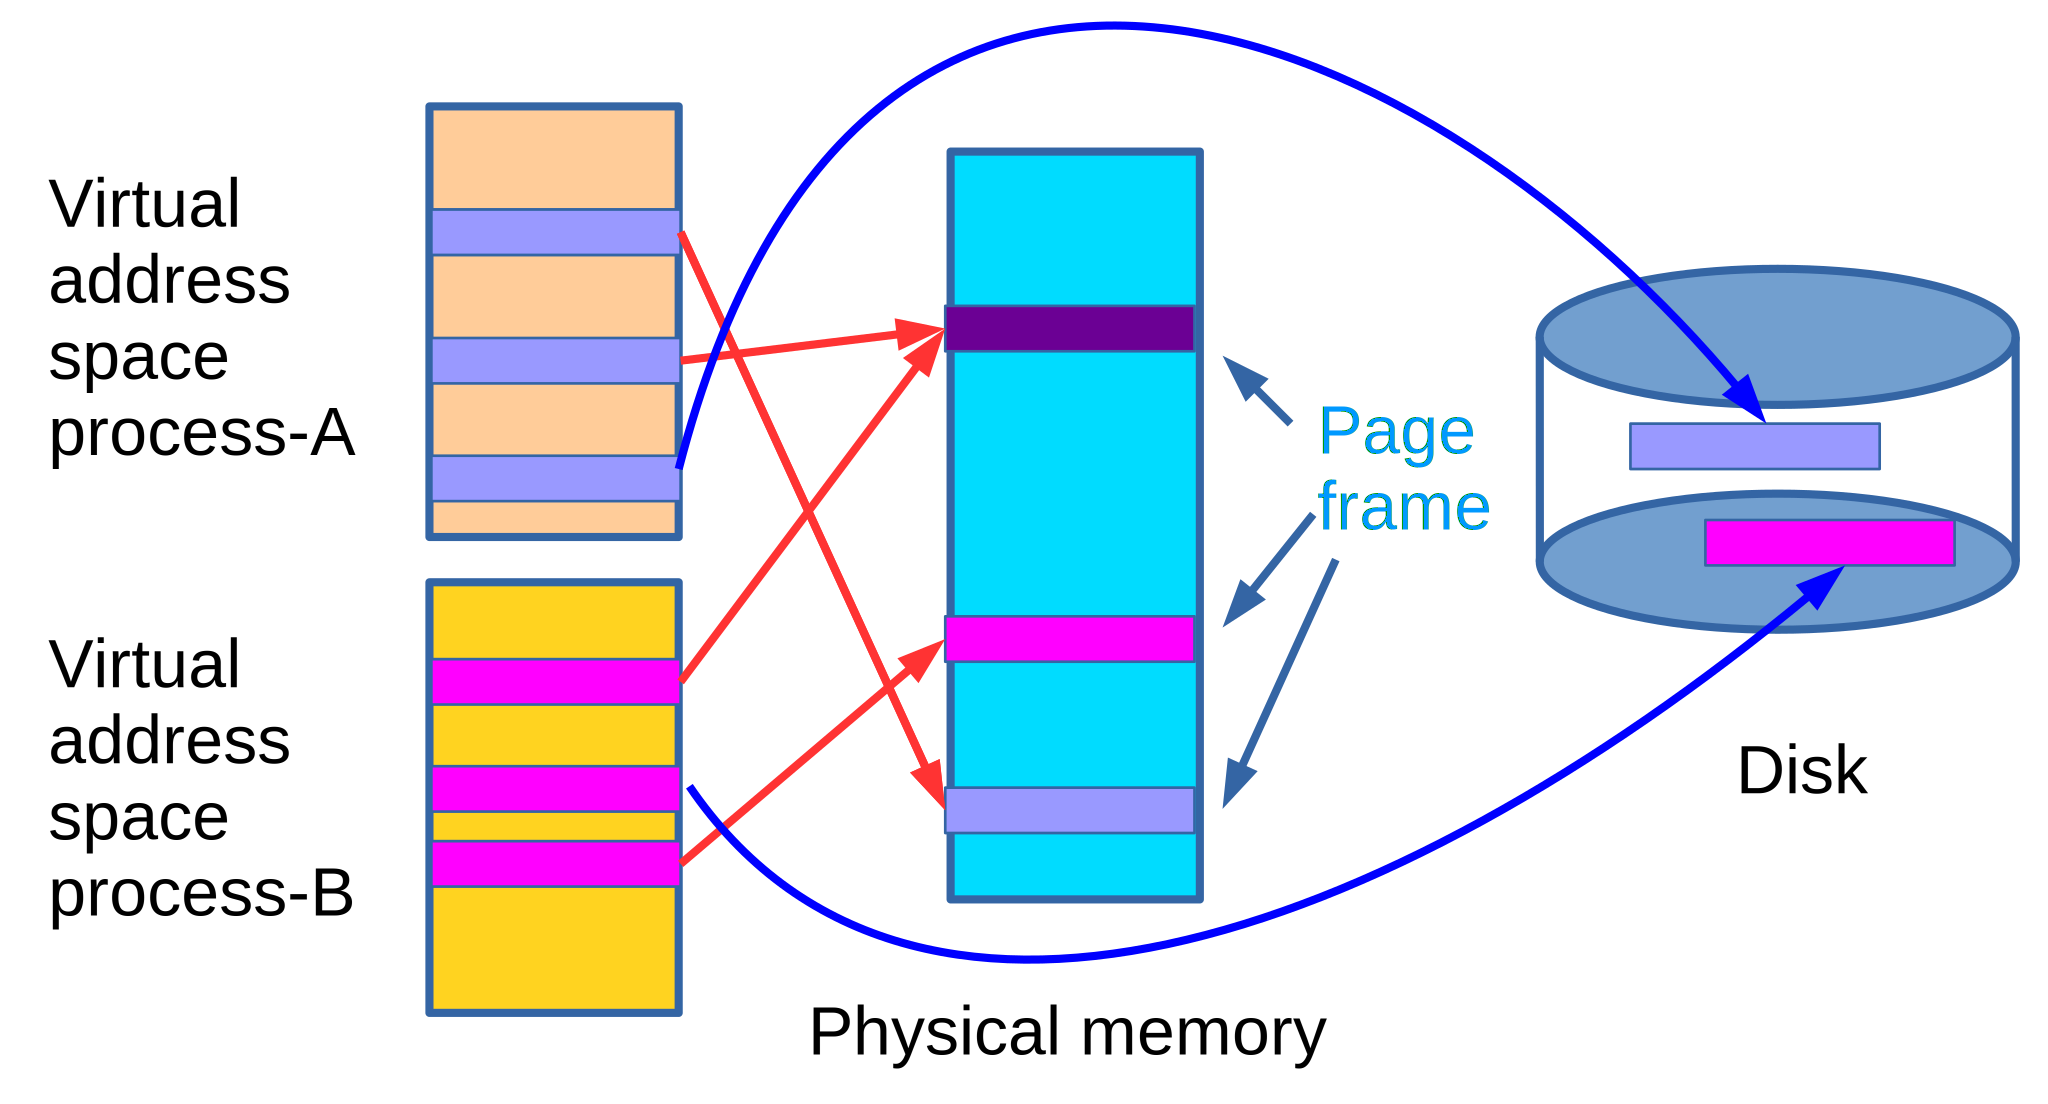
\includegraphics[width=0.80\linewidth]{paging-to-disc.pdf}

}

Translation by bytes would be expensive, space is divided into
(aligned), typically 4\,kB (sometimes larger, e.g. 64\,kB), \textbf{pages}.

\end{frame}

\begin{frame}[shrink=1]
\frametitle{Virtual to Physical Address Translation}

The translation is realized by the \textbf{Memory Management Unit} (MMU).

Translation to the pages present in memory is usually done automatically in hardware after
the operating system fills page tables and sets up the \textbf{Page Directory Base Register}
(PDBR) for given process.

On the other hand, page faults are resolved by the operating system code.
If there is access to a virtual memory area mapped into the processes and actual page is not presnet then the system reads data from the disk, network, swap partition.

As with the cache, it is necessary and challenging to find space for newly needed pages (a principle similar to LRU).

\vskip 2mm

{
\centering

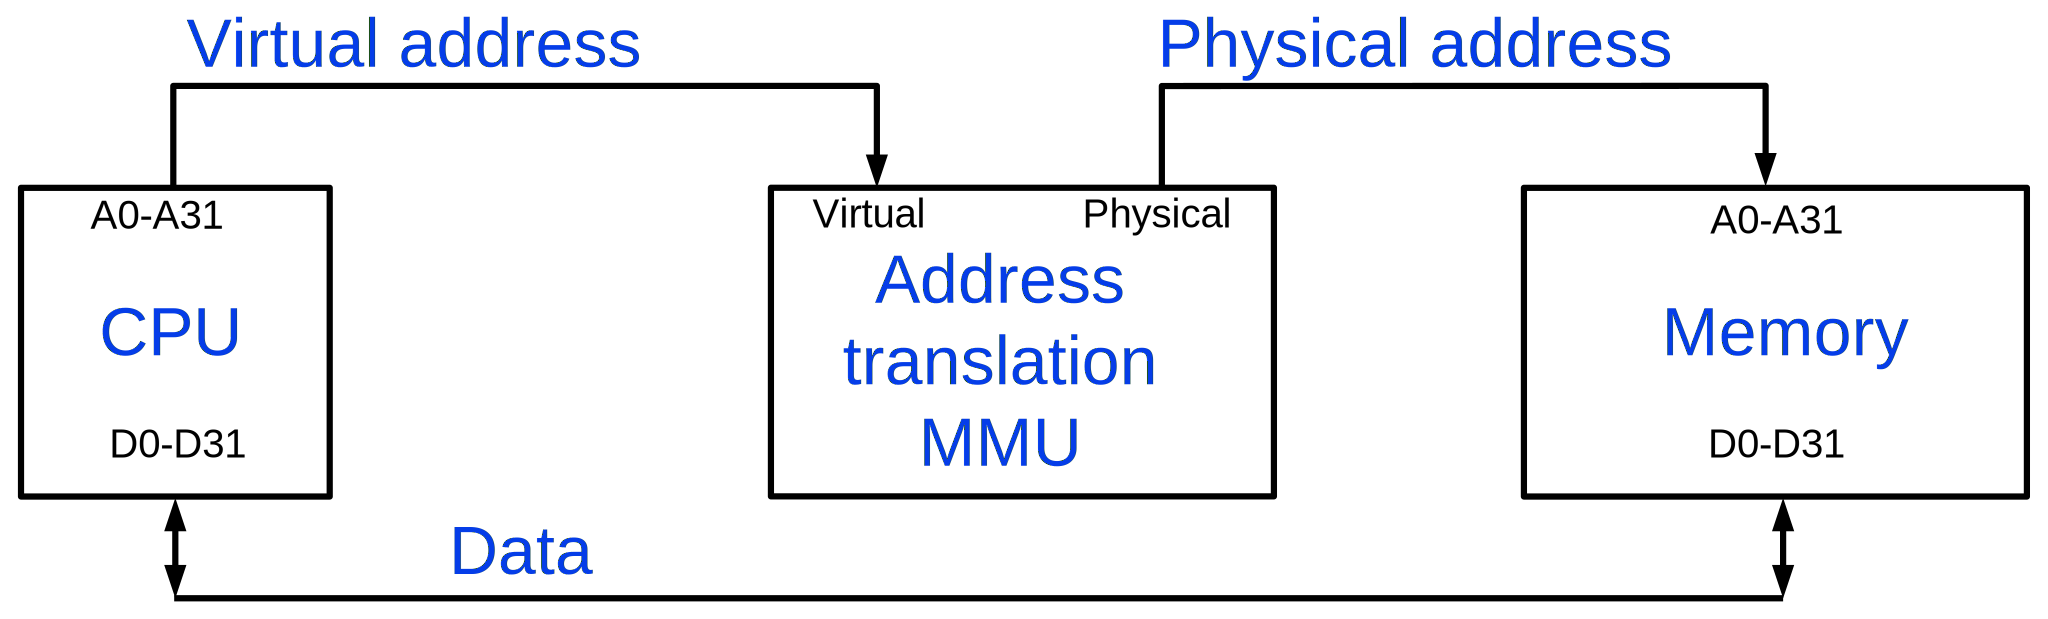
\includegraphics[width=0.80\linewidth]{paging-cpu-mm-mem.pdf}

}
\end{frame}

\begin{frame}
\frametitle{Single-level Page Table (MMU)}

{
\centering

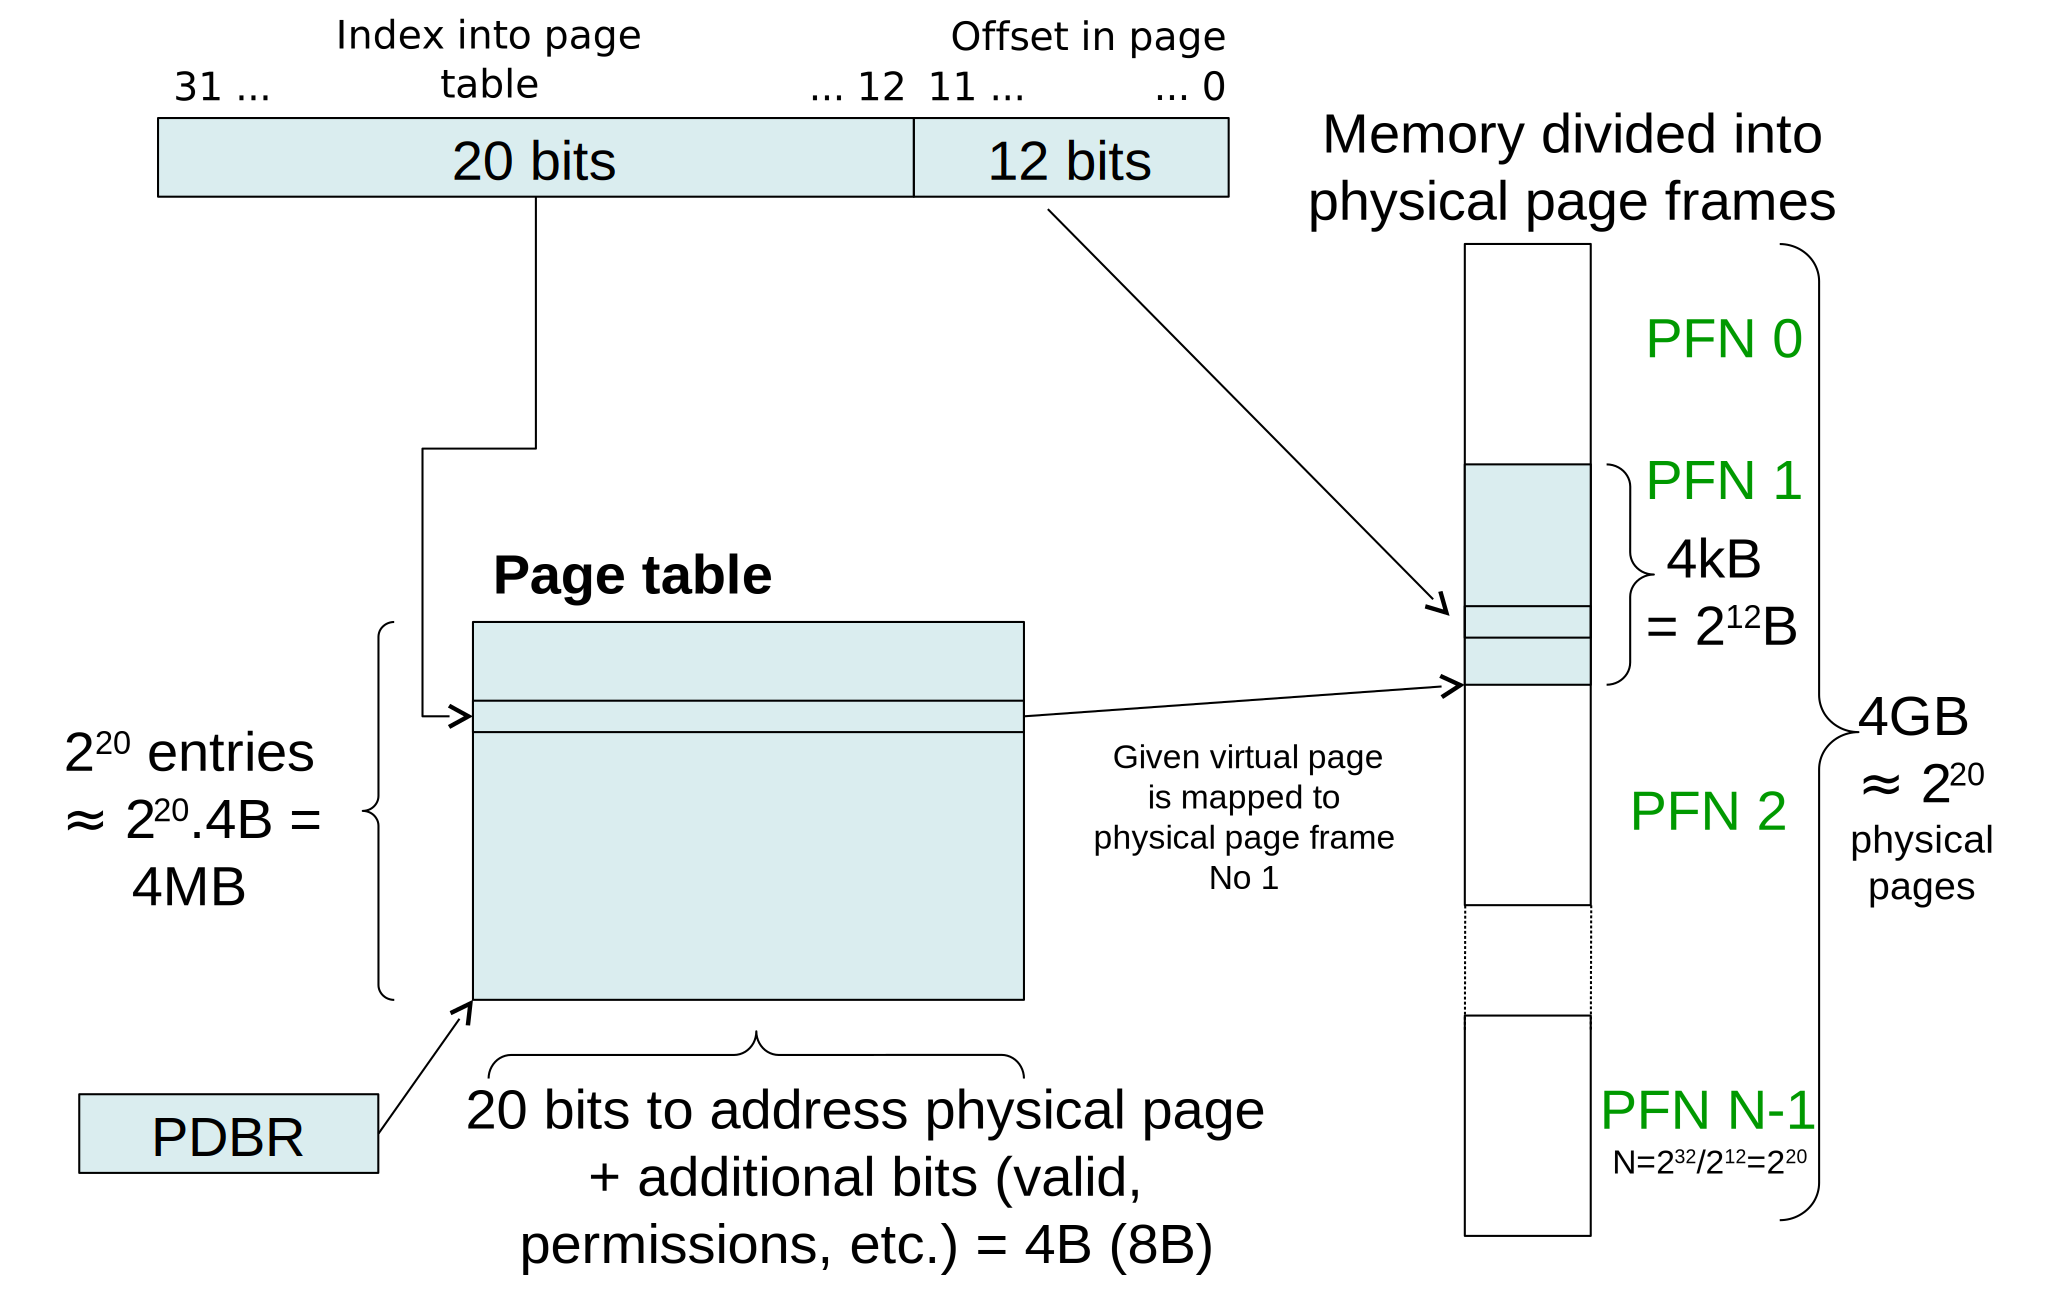
\includegraphics[width=0.80\linewidth]{paging-1-level-en.pdf}

}

Drawback of the solution, for every, even small, running process on a 32-bit
system and for 4\,kB pages, it is necessary to allocate 4\,MB (translation of 20-bit address,
4-byte entry for 32-bit physical address)

\end{frame}


\begin{frame}
\frametitle{Two-levels Page Table -- 32-bit Intel x86}

{
\centering

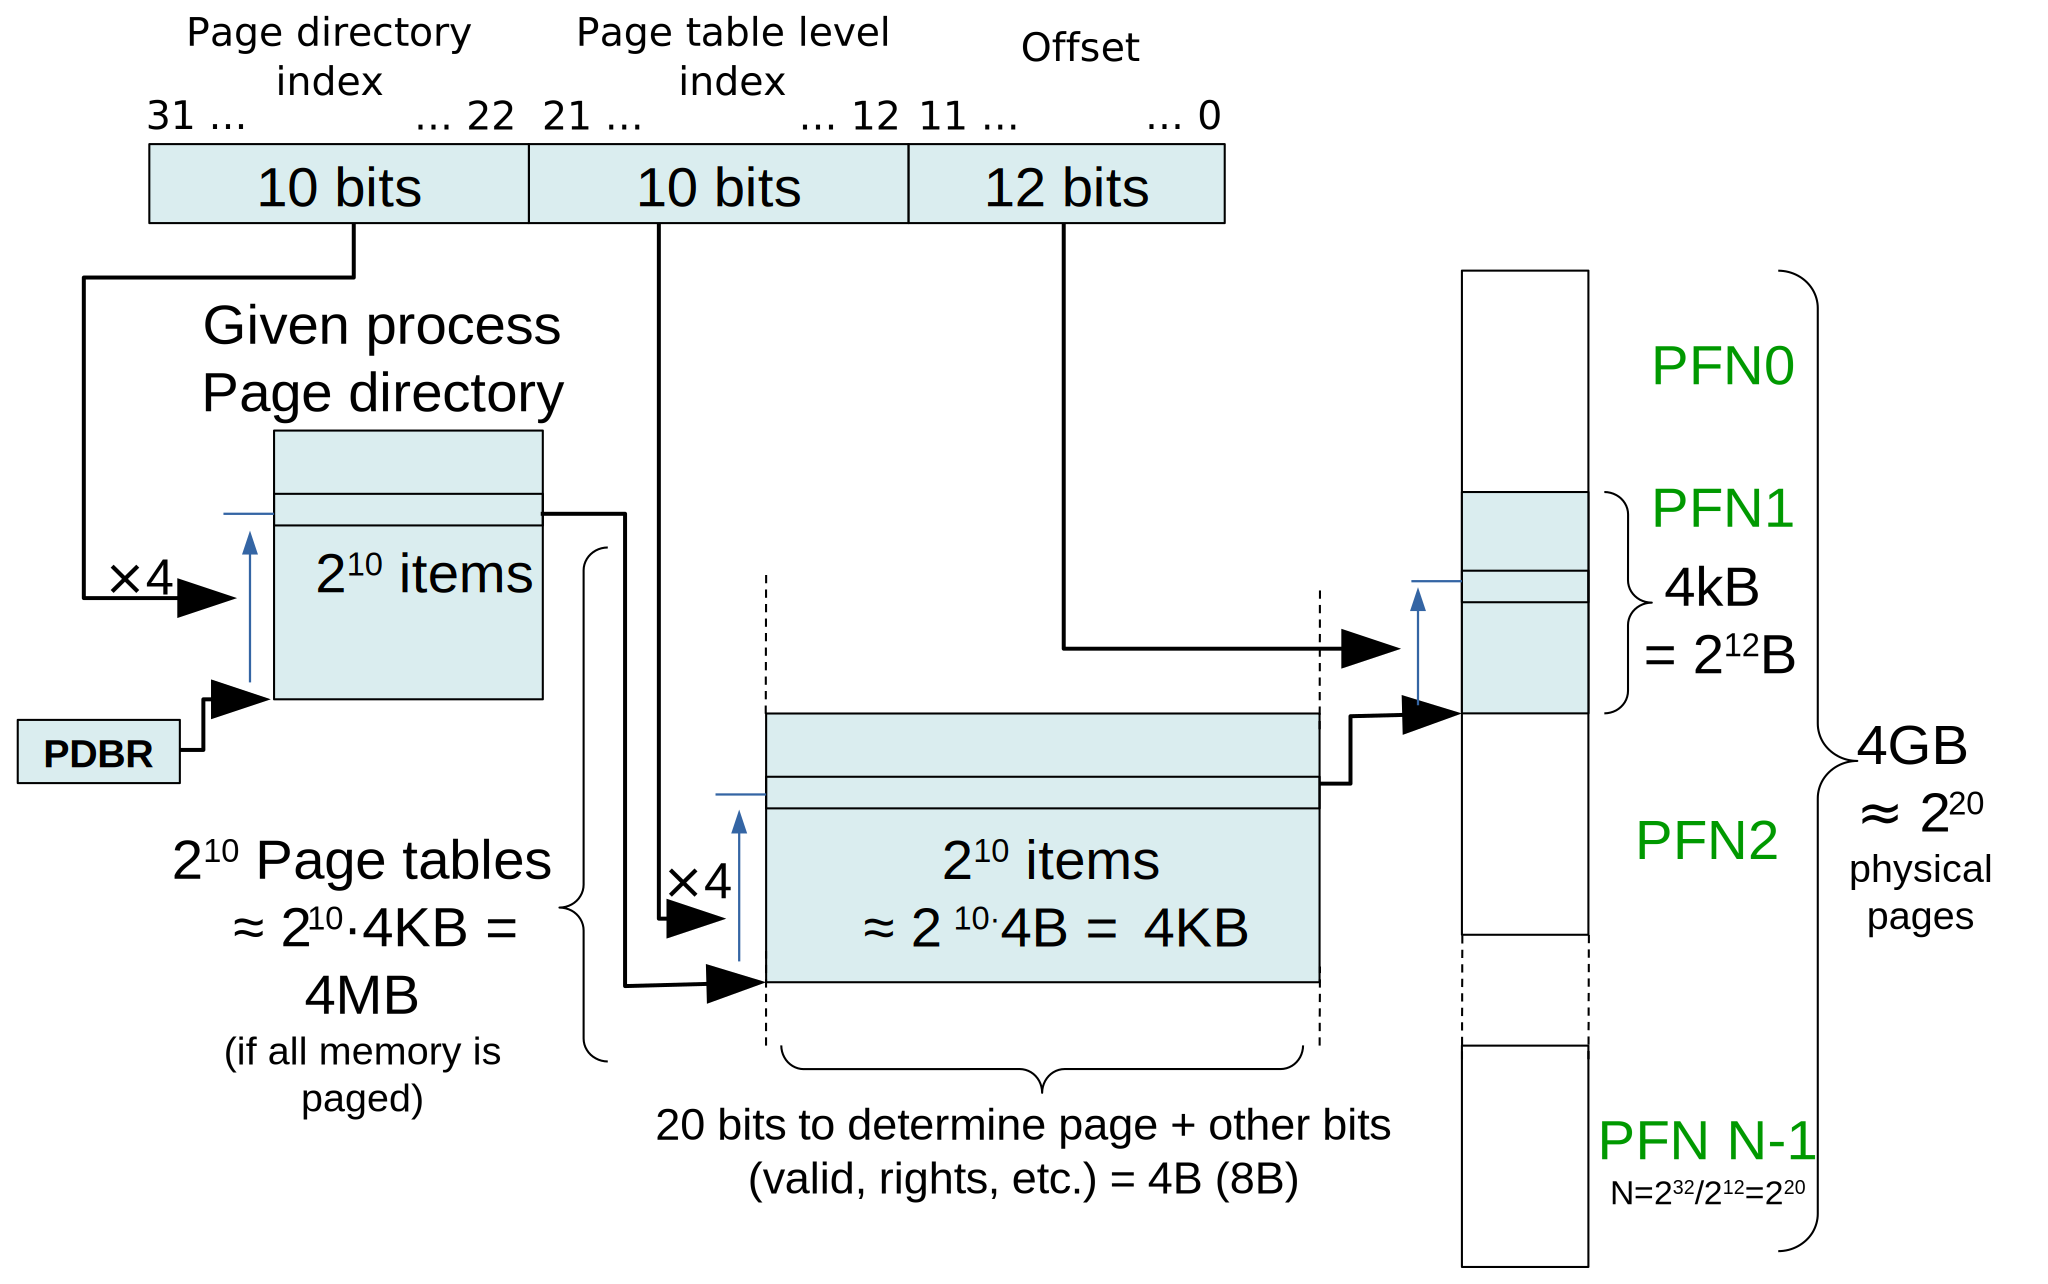
\includegraphics[width=0.65\linewidth]{paging-2-levels-en.pdf}

}

Page Directory for each process, but the second level of table with page etries is allocated only when respective virtual space area is used.

\smallskip

When translated address is divided in 10-bit groups, the array of entries
of both the directory and the table occupies to 4\,kB, same as page size. Higher-order allocations
(multiple consecutive pages) are not needed and memory management is not compicated by fragmentation.

\end{frame}

\begin{frame}
\frametitle{\textbf{Page Directory Entry} (PDE) Bit Fields}

{
\centering

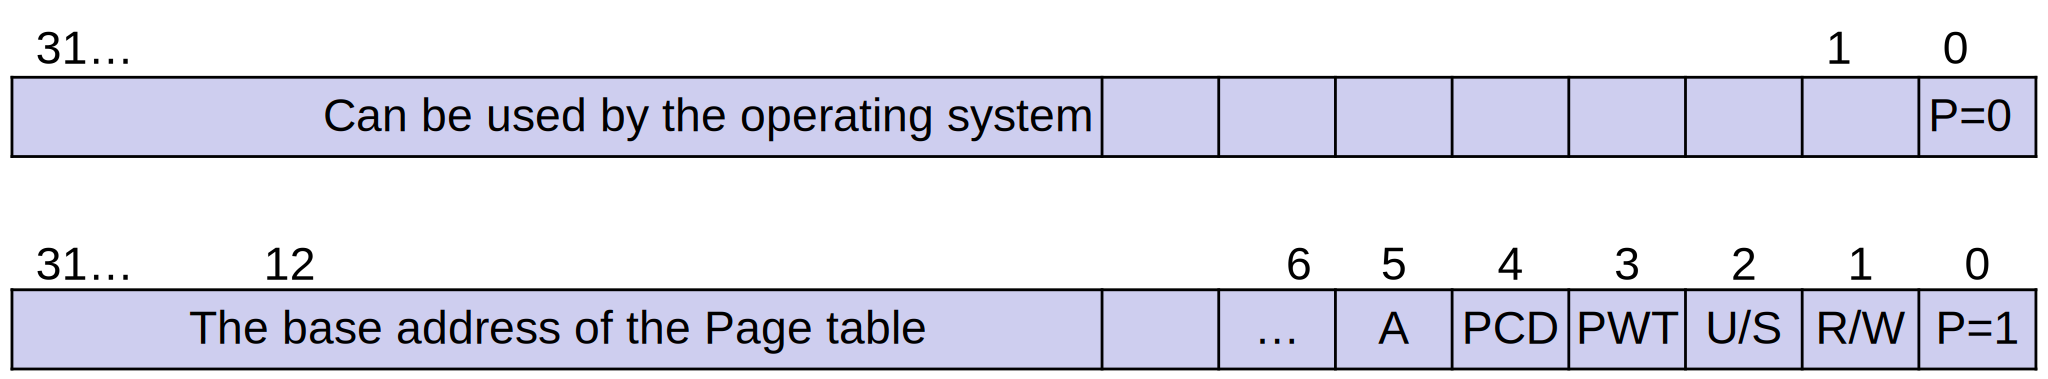
\includegraphics[width=0.90\linewidth]{paging-pde-1.pdf}

}

\vskip 2mm

\begin{itemize}
\item bit 0: Present bit -- the next level or page is presnet in physical memory (1). If it is not (0) then data are stored on disk or area is not mapped. The bit is sometimes denoted as V -- valid bit.
\item bit 1: Read/Write: 1 -- R/W -- write is permitted; 0 -- read only (RO)
\item bit 2: User/Supervisor: 1 -- user program access permitted; 0 -- only accessible by operating system
\item bit 3: Write-through/Write-back -- which method is used for writes
\item bit 4: Cache disabled/enabled -- important for memory mapped peripherals, which require immediate (uncached) registers read/write 
\item bit 5: Accessed -- set by MMU when clean and the page is accessed, used by operating system
\end{itemize}

\end{frame}

\begin{frame}
\frametitle{Final \textbf{Page Table Entry} (PTE) Bit Fields}

{
\centering

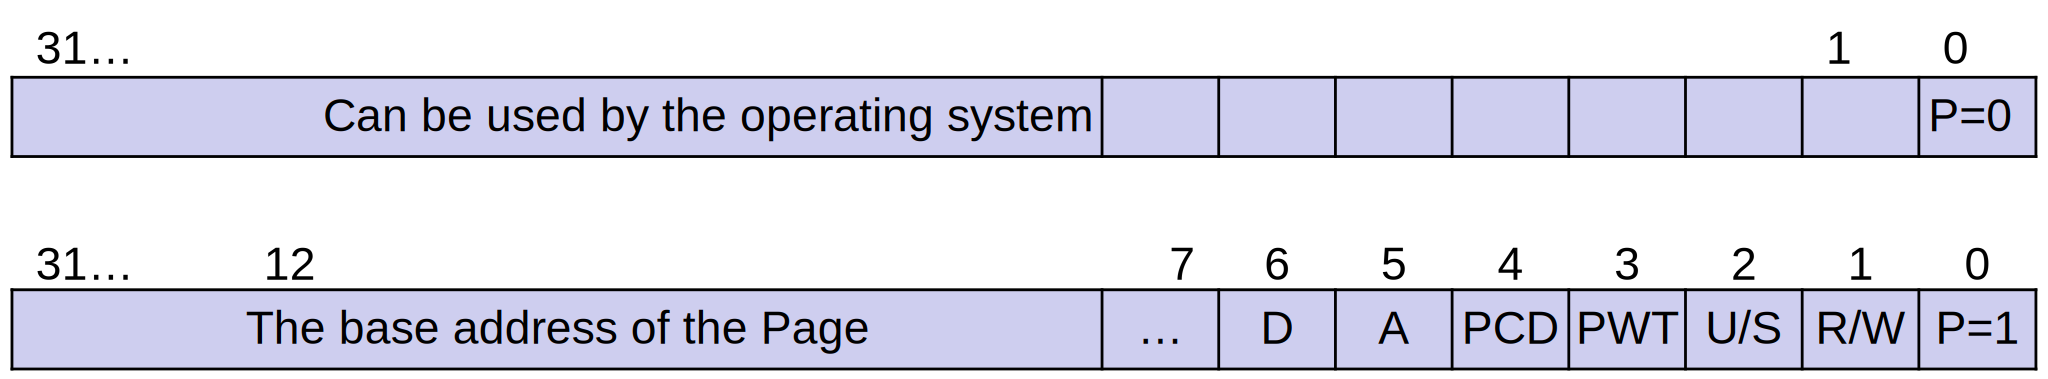
\includegraphics[width=0.90\linewidth]{paging-pte.pdf}

}

\vskip 2mm

\begin{itemize}
\item bit 6: Dirty bit, also Modified sometimes – is set by MMU if page write into page range was executed from last operating system check and the flag clear
\item The rest of flags and fields have same meaning as for page directory
\end{itemize}

\smallskip

The \textbf{Accessed} bit is crucial when the operating system searches for physical memory page frame to be released to allow it reuse for new virtual page frame.
The OS usually counts more comprehensive statistics based on these bits and zeroes them as it passes through the page frames list.
If \textbf{Dirty} bit is set, then when the physical page (PFN) is released, it is necessary to
sync the data back to the file, swap partition, etc.

\end{frame}


\begin{frame}
\frametitle{Virtual Address Translation for 64-bit CPU Architectures}

{
\centering

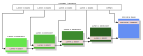
\includegraphics[width=0.90\linewidth]{address-trans-4-levels.pdf}

}

It requires multiple levels. For 64-bits and 4\,kB pages, it is theoretically
necessary to translate 52-bits. If the individual parts of the tables are sized to
fit exactly into one page and entries are 8 bytes (64 bits) each, then the translation processes 9\,bits ($512 \times 8 = 4096$) per level and thus $ceil(52 / 9) = 6$. Often, however, one to two levels are omitted, see more later.

\end{frame}

\begin{frame}
\frametitle{Speed Up (Caching) of Repeated Translation}

Each translation represents several accesses to memory, and although it is accelerated
by cache memory, it slows down operations. The \textbf{Translation Look-Aside Buffer} (TLB) is being utilized.
It works on the same principle as the memory cache, but stores a virtual address
with its translation to a physical one. Again, limited capacity, LRU, and the it needs to be taken
into account when programming.

\vskip 2mm

{
\centering

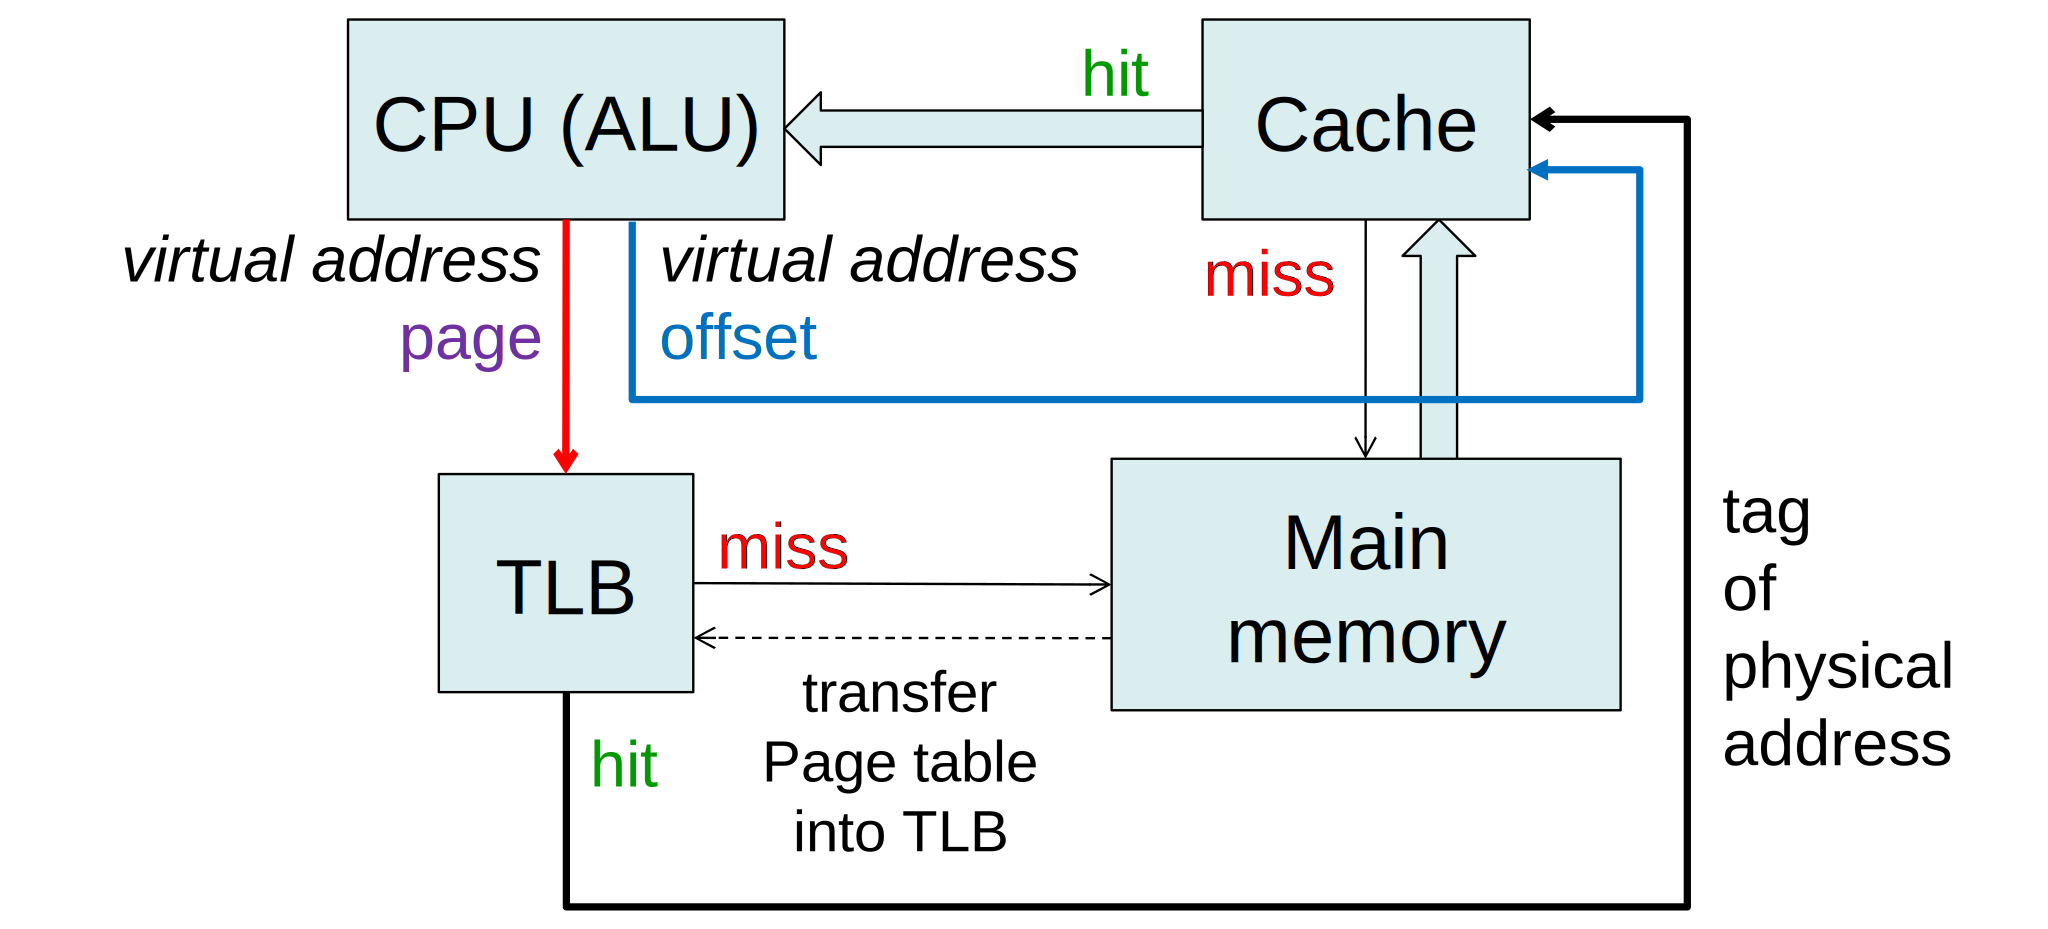
\includegraphics[width=0.80\linewidth]{paging-tlb.pdf}

}
\end{frame}

\section{Cache Memory and Paging Together}

\begin{frame}
\frametitle{Memory Subsystem on Real Chip - Intel Nehalem}

{
\centering

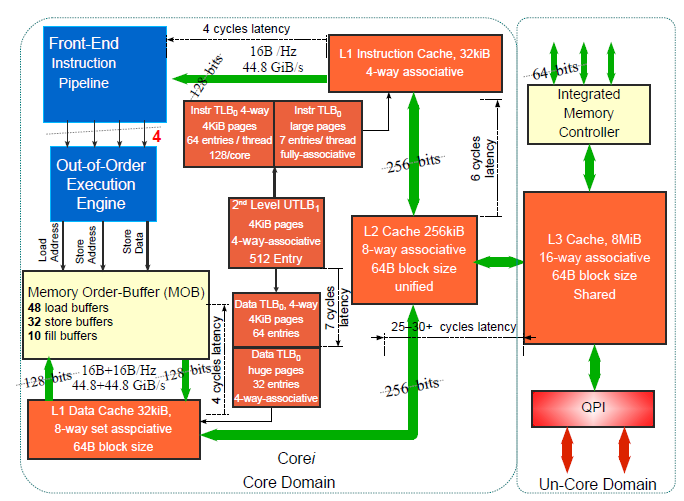
\includegraphics[width=0.80\linewidth]{fig/mem-nehalem-lat.png}

}

\end{frame}

\begin{frame}
\frametitle{Paging on 64-bit Processor Architectures}

The full 64-bit length of the physical address is not (yet) in use.
Neither is the 64-bit virtual address. Translation levels slow down the execution.
The highest address bits are replaced by the sign extension.
The top virtual memory range area is reserved for the operating system, the the bottom for applications.
Further optimization of the optional larger page -- huge pages.

{
\centering

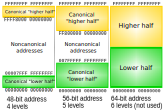
\includegraphics[width=0.6\linewidth]{paging-canonical-64-bit.pdf}

}
\end{frame}

\begin{frame}
\frametitle{Literature and Online Resources}

\begin{itemize}
\item Ulrich Drepper: \href{https://lwn.net/Articles/250967/}{What every programmer should know about memory}
\item Agner Fog: \href{https://www.agner.org/optimize/}{Software optimization resources. C++ and assembly}
\item \url{https://www.7-cpu.com/cpu/Haswell.html}
\item \url{https://www.7-cpu.com/cpu/Skylake.html}
\item WikiChips: \href{https://en.wikichip.org/wiki/amd/microarchitectures/zen}{Zen - Microarchitectures - AMD}

\end{itemize}

\end{frame}

\begin{frame}
\frametitle{Left Empty for Notes}

\end{frame}

\end{document}

